\documentclass[11pt,a4paper]{article}

% A self-contained teaching note. Compile with pdfLaTeX, BibTeX,
% pdfLaTeX, pdfLaTeX (or latexmk -pdf main.tex).
\usepackage[T1]{fontenc}
\usepackage[utf8]{inputenc}
\usepackage{lmodern}
\usepackage[english]{babel}
\usepackage{microtype}
\usepackage[a4paper,margin=29mm]{geometry}
\usepackage{amsmath,amssymb,amsthm,mathtools}
\usepackage{booktabs,array}
\usepackage{etoolbox}
\usepackage{fancyhdr}
\usepackage{tikz}
\usepackage{caption}
\usepackage{float}
\usepackage{needspace}
\usepackage{hyperref}
\hypersetup{colorlinks=true,linkcolor=black,citecolor=black,urlcolor=black,
  pdfauthor={Osvaldo L. Santos-Pereira},
  pdftitle={A Tenth-Degree Polynomial Equation: Roots of Unity, Cyclotomic Factorization, and Root Multiplicities of Products of Geometric Sums}}
\usetikzlibrary{calc}
\captionsetup{font=small,labelfont=bf}
\setlength{\parindent}{1.4em}
\setlength{\parskip}{0.18em}
\allowdisplaybreaks[2]
\emergencystretch=2em
\numberwithin{equation}{section}

% Upright theorem bodies support prose exposition, including definitions.
\newtheoremstyle{uprightpaper}{8pt}{8pt}{\normalfont}{}{\bfseries}{.}{0.65em}{}
\theoremstyle{uprightpaper}
\newtheorem{theorem}{Theorem}[section]
\newtheorem{proposition}{Proposition}[section]
\newtheorem{lemma}{Lemma}[section]
\newtheorem{corollary}{Corollary}[section]
\newtheorem{definition}{Definition}[section]
\newtheorem{remark}{Remark}[section]
\newtheorem{example}{Example}[section]
\renewcommand{\qedsymbol}{$\square$}
% A small geometric terminal symbol marks the end of each formal definition.
% It is placed within the environment, on the closing line of prose.
\newcommand{\definitionmark}{\unskip\nobreak\hfill\ensuremath{\lozenge}}
\AtEndEnvironment{definition}{\leavevmode\definitionmark}

% Running heads and feet: the section heading is set in lower case.
\pagestyle{fancy}
\fancyhf{}
\renewcommand{\sectionmark}[1]{\markboth{\thesection.\ \MakeLowercase{#1}}{\thesection.\ \MakeLowercase{#1}}}
\renewcommand{\subsectionmark}[1]{}
\fancyhead[L]{\small\nouppercase{\rightmark}}

\fancyfoot[C]{\footnotesize\thepage}
\renewcommand{\headrulewidth}{0.4pt}
\renewcommand{\footrulewidth}{0.4pt}
\setlength{\headheight}{14pt}
\fancypagestyle{plain}{%
  \fancyhf{}
  \fancyhead[L]{\small\nouppercase{\rightmark}}
  
  \fancyfoot[C]{\footnotesize\thepage}
  \renewcommand{\headrulewidth}{0.4pt}
  \renewcommand{\footrulewidth}{0.4pt}}


\newcommand{\C}{\mathbb{C}}
\newcommand{\R}{\mathbb{R}}
\newcommand{\Q}{\mathbb{Q}}
\newcommand{\Z}{\mathbb{Z}}
\newcommand{\ord}{\operatorname{ord}}
\newcommand{\card}{\operatorname{card}}
\newcommand{\gcdpoly}{\operatorname{gcd}}
\newcommand{\ind}{\mathbf{1}}
\newcommand{\Sm}{S_m}
\newcommand{\Pm}{P_{m,b}}
\newcommand{\Um}{\mathcal{U}}
\newcommand{\mult}{\operatorname{mult}}
\newcommand{\Pmk}{P_{m,b,k}}

\title{A Tenth-Degree Polynomial Equation:\\
Roots of Unity, Cyclotomic Factorization, and Root Multiplicities of Products of Geometric Sums}
% Author details are kept in macros and displayed beneath the name.
\newcommand{\AuthorName}{Osvaldo L. Santos-Pereira}
\newcommand{\AuthorEmail}{olsp@if.ufrj.br}
\newcommand{\AuthorOrcid}{0000-0003-2231-517X}
\newcommand{\AuthorAffiliation}{Physics Institute, Universidade Federal do Rio de Janeiro (UFRJ)}
\author{\AuthorName\\[2pt]
\small ORCID: \href{https://orcid.org/\AuthorOrcid}{\AuthorOrcid}
\quad E-mail: \href{mailto:\AuthorEmail}{\AuthorEmail}\\[2pt]
\small \AuthorAffiliation}
\date{}

% Compact front matter; the document's body typography is unchanged.
\makeatletter
\renewcommand{\maketitle}{%
  \thispagestyle{plain}%
  \begingroup
    \setlength{\parindent}{0pt}%
    \setlength{\parskip}{0pt}%
    \centering
    {\LARGE \@title\par}%
    \vspace{6pt}%
    {\normalsize \@author\par}%
  \endgroup
  \vspace{6pt}%
}
\makeatother
\renewenvironment{abstract}{%
  \par\begingroup\small
  \setlength{\parskip}{0pt}%
  \begin{center}\bfseries Abstract\end{center}%
  \vspace{-4pt}\noindent\ignorespaces
}{\par\endgroup\vspace{5pt}}

\begin{document}
\maketitle
\begin{abstract}
This teaching note develops the algebraic ideas needed to solve a tenth-degree polynomial equation with vanishing coefficients at $x^3$ and $x^7$ and then extends the same methods to products of finite geometric sums. The motivating polynomial factors as $P(x)=S_3(x)S_3(x^4)=\Phi_3(x)^2\Phi_6(x)\Phi_{12}(x)$ and has eight distinct zeros: six simple roots and two double roots, the latter being the primitive cube roots of unity. Roots of unity, multiplicative order, Euler's totient function, cyclotomic factorization, Vi\`ete's formulas, and reciprocal reduction are developed as needed. For the general product $Q_{m,n,b}(x)=S_m(x)S_n(x^b)$, the number of double roots is $\gcd(m,nb)-\gcd(m,b)$ and the number of distinct roots is $(m-1)+b(n-1)$ minus this overlap. A parity criterion gives the existence and multiplicity of the only possible real root, $-1$.
\end{abstract}
\begingroup\small
\noindent\textbf{Keywords:} polynomials; roots of unity; cyclotomic polynomials; root multiplicity; finite geometric series; products of geometric sums; greatest common divisor; reciprocal polynomials; Chebyshev polynomials; Dickson polynomials; Vi\`ete's formulas; worked problems.\par
\noindent\textbf{Mathematics Subject Classification (2020):} 11C08; 11R18; 12E10; 11A25; 33C45; 97H20.
% Suggested arXiv classification: primary math.HO; cross-list math.NT.

\par\endgroup

% Related entries share a row, without removing any original symbol.
\par\vspace{7pt}
\noindent{\large\bfseries Glossary of notation}\par
\markboth{glossary of notation}{}
\vspace{4pt}
\begingroup
\small
\setlength{\parskip}{0pt}
\renewcommand{\arraystretch}{1.16}
\setlength{\tabcolsep}{0pt}
\noindent
\begin{tabular}{@{}>{\raggedright\arraybackslash}p{0.27\linewidth}@{\hspace{1em}}>{\raggedright\arraybackslash}p{\dimexpr0.73\linewidth-1em\relax}@{}}
\toprule
Symbol & Definition and interpretation\\
\midrule
$\C,\R,\Q,\Z;\ \C^\times$ & Complex, real, rational, and integer numbers; $\C^\times=\C\setminus\{0\}$\\
$F(x),\deg F,Z(F)$ & Polynomial, its degree, and its zero set\\
$\mult_F(\alpha)$ & Root multiplicity; zero when $F(\alpha)\ne0$\\
$e_j$ & Elementary symmetric sum of order $j$, counting multiplicities\\
$\mathbf 1_A$ & Indicator of a condition or set $A$\\
$\omega_{n,h};\ \omega_n,\omega$ & $e^{2\pi i h/n}$, $0\le h<n$; $\omega_n=\omega_{n,1}$ for $n\ge2$, and $\omega=\omega_3$\\
$\mathcal U_n,\ord(z)$ & Set of $n$-th roots of unity; multiplicative order of $z$\\
$\gcd(a,b)$ & Greatest common divisor of the integers $a$ and $b$\\
$\overline z,|z|,\arg z$ & Complex conjugate, modulus, and argument (the latter for $z\ne0$)\\
$\varphi(n)$ & Euler's totient function\\
$\Phi_n(x)$ & $n$-th cyclotomic polynomial\\
$S_m(x)$ & Finite geometric sum $1+x+\cdots+x^{m-1}$\\
$P_{m,b}(x)$ & Equal-length product $S_m(x)S_m(x^b)$\\
$Q_{m,n,b}(x)$ & Unequal-length product $S_m(x)S_n(x^b)$\\
$P(x)$ & Motivating polynomial $P_{3,4}(x)$\\
$u$ & Substitution $u=x^4$\\
$t,\tau(x)$ & Reciprocal variable and map: $t=\tau(x)=x+x^{-1}$, $x\ne0$\\
$T_j$ & Chebyshev polynomial of the first kind\\
$D_j(t,1)$ & Dickson polynomial: $D_j(x+x^{-1},1)=x^j+x^{-j}$\\
$R(t)$ & Reduced polynomial obtained from $x^{-5}P(x)$\\
$\delta_{m,n,b},\nu_{m,n,b}$ & Numbers of double and distinct roots of $Q_{m,n,b}$\\
$\Theta_\pm$ & Angle sets from the substitution $u=x^4$\\
\bottomrule
\end{tabular}
\par\endgroup
\clearpage

\section{Introduction}\label{sec:intro}

Polynomial equations connect algebraic factorizations with the geometry of the complex plane. The fundamental theorem of algebra determines the number of complex roots, including multiplicities. The factor theorem and the relationship between roots and coefficients provide methods for identifying and verifying them. Certain exponent patterns yield factorizations into finite geometric sums, and the complex zeros of these sums are roots of unity. This correspondence between algebraic factors and points on the unit circle forms the basis of the note~\cite{barbeau1989,andreescu2014,needham1997}.

Roots of unity form finite cyclic sets under multiplication. Their multiplicative orders classify the primitive roots, and Euler's totient function counts the roots of each exact order. Cyclotomic polynomials collect these roots into monic factors over the integers. The relation between roots of unity, integer divisibility, and cyclotomic factorization is established in standard treatments of algebra and number theory~\cite{dummit2004,hardywright2008,irelandrosen1990,washington1997}. The examples developed here include the complete calculation of the first twelve cyclotomic polynomials and a classification of all twelve roots of the equation $z^{12}=1$.

The exposition begins with polynomials and factorization in Section~\ref{sec:polytheory}, followed by roots of unity, the totient function, and cyclotomic polynomials in Section~\ref{sec:rootsunity}. Section~\ref{sec:applications} solves the motivating equation using exponent blocks, complex root geometry, substitution, and Vi\`ete's formulas. Section~\ref{sec:chebyshev-applications} develops the reciprocal reduction and the general root-counting formulas for products of geometric sums. Section~\ref{sec:exercise-section} contains worked exercises, followed by the conclusion.

\section{Polynomials}\label{sec:polytheory}

This section establishes the algebraic tools needed to analyze the roots of a polynomial. We define polynomial degree and root multiplicity, derive the factorization of a complex polynomial into linear factors, and relate the coefficients to its roots. The derivative criterion identifies repeated roots, reciprocal symmetry provides a method of reducing certain even-degree equations, and finite geometric sums yield explicit factorization identities. We use these results to determine and verify the solutions discussed in Section~\ref{sec:applications}.

\subsection{Algebraic foundations}\label{subsec:polynomial-foundations}

A polynomial is a finite linear combination of nonnegative integer powers of a variable. Its algebraic properties are encoded in the coefficients, degree, and factorization. We first fix the terminology used in the sequel, including the distinction between distinct zeros and zeros counted with multiplicity. The root-factorization and coefficient identities are standard results of polynomial algebra (see Refs.~\cite{barbeau1989, dummit2004}).

\begin{definition}[Polynomial and degree]\label{def:polynomial}
Let $K$ be a field. A polynomial over $K$ is a formal expression
\begin{equation}\label{eq:polynomial}
 F(x)=a_0+a_1x+\cdots+a_dx^d,\qquad
 a_j\in K,\quad a_d\neq0.
\end{equation}
Its degree is $d$, its leading coefficient is $a_d$, and its constant coefficient is $a_0$. A polynomial is \emph{monic} when $a_d=1$. For $\alpha\in K$, the value $F(\alpha)$ is obtained by evaluation, and $\alpha$ is a root if $F(\alpha)=0$.
\end{definition}

The factor theorem states that $F(\alpha)=0$ precisely when $x-\alpha$
divides $F(x)$. Repeated divisibility by the same linear polynomial gives
the multiplicity of the root. This distinction is necessary whenever two
factorizations share a root.

\begin{definition}[Root multiplicity]\label{def:mult}
If $F(\alpha)=0$, the multiplicity $r$ of $\alpha$ is the unique positive integer such that $F(x)=(x-\alpha)^rH(x)$ with $H(\alpha)\neq0$. We write $\mult_F(\alpha)=r$, and set $\mult_F(\alpha)=0$ when $F(\alpha)\neq0$. Multiplicity one is called \emph{simple}, and multiplicity two is called \emph{double}.
\end{definition}

For a product $F=GH$, the factor theorem gives $\mult_F(\alpha)=\mult_G(\alpha)+\mult_H(\alpha)$. The fundamental theorem of algebra asserts that a nonconstant polynomial of degree $d$ over $\C$ factors into $d$ linear factors, counted with multiplicity~\cite{dummit2004,needham1997}. For a monic polynomial with complex roots $r_1,\ldots,r_d$, these two conclusions are summarized by
\begin{equation}\label{eq:fta-factorization}
 F(x)=\prod_{j=1}^{d}(x-r_j),\qquad
 \sum_{\alpha:\,F(\alpha)=0}\mult_F(\alpha)=d.
\end{equation}
The repetition of a root in the product is therefore equivalent to multiplicity greater than one. The coefficient relations of Vi\`ete follow by expanding the linear factorization; they are stated in full in Proposition~\ref{prop:viete} and later provide an independent check on the original polynomial's roots~\cite{barbeau1989}. A derivative can detect repeated roots. In characteristic zero, the factor $(x-\alpha)^r$ contributes $(x-\alpha)^{r-1}$ to the derivative, so $\alpha$ is repeated precisely when $F(\alpha)=F'(\alpha) = 0$. Accordingly, $F$ is \emph{square-free} when all its complex roots are simple, or equivalently when the monic greatest common divisor of $F$ and $F'$ is one~\cite[Section~13.5]{dummit2004}. This criterion distinguishes repeated roots from simple roots in the applications below.

\begin{definition}[Reciprocal polynomial]\label{def:reciprocal}
A polynomial $F$ of degree $d$ with nonzero constant coefficient is \emph{reciprocal} when $x^dF(x^{-1})=F(x)$ for every $x\neq0$. Equivalently, its coefficients satisfy $a_j=a_{d-j}$. Its nonzero roots occur in inverse pairs, with multiplicities preserved.
\end{definition}

For reciprocal polynomials of even degree, the substitution $t=x+x^{-1}$ transforms paired powers $x^j+x^{-j}$ into polynomials in $t$. We develop this reduction in Section~\ref{sec:reciprocalmethod} and relate it to the Chebyshev recurrence~\cite{needham1997}.


\subsection{Finite geometric sums}\label{subsec:geometric}

The product of a polynomial with a linear factor can produce a telescoping sum. For every integer $m\ge 2$, define the finite geometric sum $S_m$ as the polynomial with all coefficients equal to one from degree zero to degree $m-1$. Subtracting its shifted copy gives
\begin{align}
 S_m(x)&=1+x+\cdots+x^{m-1},\label{eq:geomsum-basic}\\
 (x-1)S_m(x)&=x^m-1,\qquad S_m(1)=m.\label{eq:geomsum-telescoping}
\end{align}
For $x\ne1$, Equation~\eqref{eq:geomsum-telescoping} yields $S_m(x)=(x^m-1)/(x-1)$. The expression $S_m(1)=m$ must be evaluated using the polynomial definition, because the quotient has a removable singularity there. The roots of $S_m$ are characterized in Corollary~\ref{cor:geomsum-cyclotomic} after roots of unity and cyclotomic polynomials have been introduced. These relations are the standard finite geometric-series identities (see Ref.~\cite{barbeau1989}); divisibility properties of such sums are studied in Ref.~\cite{hartwig2023divisibility}.

\Needspace{17\baselineskip}
\section{Roots of unity}\label{sec:rootsunity}

The solutions of equations of the form $z^n=1$ can be described using complex numbers, their polar representation, and the multiplication of complex numbers on the unit circle. This section develops that description from the definitions of modulus and argument, derives all $n$-th roots of unity, and establishes their simplicity. The multiplicative order of a root then leads to Euler's totient function and the decomposition of $x^n-1$ into cyclotomic polynomials. These concepts will determine both the positions and the multiplicities of the solutions studied in Section~\ref{sec:applications}~\cite{andreescu2014,needham1997,irelandrosen1990}.

\subsection{Complex representation and roots of unity}\label{subsec:complex-roots}

The complex numbers extend the real numbers by adjoining a unit $i$ with $i^2=-1$. Every $z\in\C$ has unique real coordinates $a$ and $b$ such that $z=a+ib$. Identifying $z$ with the point $(a,b)$ makes addition a vector operation in the complex plane. Multiplication admits a geometric interpretation through polar coordinates: the moduli multiply, while the arguments add~\cite{needham1997,andreescu2014}.

\begin{definition}[Conjugate, modulus, and argument]\label{def:complex-polar}
For $z=a+ib\in\C$, its \emph{complex conjugate} and \emph{modulus} are, respectively, \begin{equation}\label{eq:complex-modulus} \overline z=a-ib,\qquad |z|=\sqrt{z\overline z}=\sqrt{a^2+b^2}.
\end{equation}
For $z\neq0$, an \emph{argument} of $z$ is a real angle $\theta$ satisfying $a=|z|\cos\theta$ and $b=|z|\sin\theta$. With $r=|z|>0$, the \emph{polar representation} is 
\begin{equation}\label{eq:complex-polar}
 z=r(\cos\theta+i\sin\theta)=r e^{i\theta}.
\end{equation}
Arguments differing by an integer multiple of $2\pi$ represent the same complex number.
\end{definition}

Euler's formula in Equation~\eqref{eq:complex-polar} converts angular addition into multiplication: $e^{i\alpha}e^{i\beta}=e^{i(\alpha+\beta)}$. Consequently, taking the $n$-th power of a point on the unit circle multiplies its argument by $n$. This is De Moivre's formula, which for any integer $n\geq1$ takes the form
\begin{equation}\label{eq:de-moivre}
 (\cos\theta+i\sin\theta)^n=\cos(n\theta)+i\sin(n\theta).
\end{equation}
The formula supplies a direct method for solving equations that prescribe
a positive integer power of a complex number.

\begin{definition}[Root of unity]\label{def:rootsunity}
For a positive integer $n$, a complex number $z$ is an \emph{$n$-th root
of unity} when it satisfies the equation
\begin{equation}\label{eq:unity-equation}
 z^n=1.
\end{equation}
The set of all such numbers is denoted by $\mathcal U_n$.
\end{definition}

To solve Equation~\eqref{eq:unity-equation}, take the modulus of both sides. The identity $|z^n|=|z|^n$ implies $|z|=1$, so each solution has the form $z=e^{i\theta}$ for some real angle $\theta$. Applying Equation~\eqref{eq:de-moivre} shows that the power equals one precisely when its angle is an integer multiple of a complete revolution, that is,
\begin{equation}\label{eq:unity-angles}
 z^n=1\quad\Longleftrightarrow\quad n\theta=2\pi h,
 \qquad h\in\Z,\quad z=e^{i\theta}.
\end{equation}
Two integers $h$ produce the same solution exactly when their difference is divisible by $n$. Choosing the representatives $h=0,\ldots,n-1$ therefore yields all $n$ distinct values. We denote the indexed solutions by
\begin{equation}\label{eq:rootsunity}
 \omega_{n,h}=e^{2\pi i h/n}
 =\cos\left(\frac{2\pi h}{n}\right)
 +i\sin\left(\frac{2\pi h}{n}\right),
 \qquad h=0,1,\ldots,n-1.
\end{equation}
Equation~\eqref{eq:rootsunity} places the roots at the vertices of a regular $n$-gon on the unit circle, with angular separation $2\pi/n$. For $n\geq2$, we write $\omega_n=\omega_{n,1}=e^{2\pi i/n}$; every $n$-th root equals $\omega_n^h$ for one of the indicated indices. In the important cubic case, we abbreviate $\omega:=\omega_3=e^{2\pi i/3}$. The roots of the cubic equation are $\mathcal U_3=\{1,\omega,\omega^2\}$, while the fourth roots are $\mathcal U_4 = \{1,i,-1,-i\}$. By Equation~\eqref{eq:geomsum-telescoping}, the two nontrivial cubic roots satisfy $1+\omega+\omega^2 = 0$.

Finally, the solutions in Equation~\eqref{eq:rootsunity} are simple roots of the polynomial $x^n-1$. Indeed, its derivative is $nx^{n-1}$, and a root of unity is nonzero; thus the polynomial and its derivative cannot vanish at the same point. This verifies the root count and ensures that any repeated root in a subsequent product arises from factors sharing a zero, not from the individual equation $z^n=1$~\cite{dummit2004}.

\subsection{Order and Euler's totient function}\label{subsec:order-totient}

The order of a root of unity is the least positive exponent for which it becomes one. This integer identifies the cyclotomic factor containing that root. We begin by defining order and proving its basic divisibility property.

\begin{definition}[Order and primitivity]\label{def:order}
The \emph{order} of a root of unity $z$ is the least positive integer $d$ such that $z^d=1$. A root of order $d$ is called a \emph{primitive $d$-th root of unity}. This terminology organizes the cyclotomic factors introduced below~\cite{hardywright2008,irelandrosen1990}.
\end{definition}
\begin{lemma}[Order divides every exponent]\label{lem:order-divides}
If $z^n=1$ and $\ord(z)=d$, then $d\mid n$.
\end{lemma}
\begin{proof}
By Euclidean division, write $n=qd+r$ with $0\leq r<d$. Then $z^r=z^n(z^d)^{-q}=1$. The minimality of $d$ forces $r=0$, so $d\mid n$.
\end{proof}


\begin{definition}[Relatively prime integers and Euler's totient function]\label{def:totient}
The greatest common divisor $\gcd(a,b)$ of two integers, not both zero, is the largest positive integer dividing both $a$ and $b$. Two integers are \emph{relatively prime} (or \emph{coprime}) if $\gcd(a,b)=1$; equivalently, their only positive common divisor is $1$. For example, $5$ and $12$ are relatively prime, whereas $6$ and $12$ are not. For every integer $n\geq1$, Euler's totient function counts the integers $h$ between $1$ and $n$ that are relatively prime to $n$:
\begin{equation}\label{eq:totient-def}
\varphi(n)=\#\{h\in\{1,\ldots,n\}:\gcd(h,n)=1\}, \qquad\varphi(1)=1.
\end{equation}
Equivalently, $\varphi(n)$ counts the primitive $n$-th roots of unity.
\end{definition}

The totient can be computed by excluding integers divisible by each prime divisor. If $p$ runs through the distinct primes dividing $n$, inclusion--exclusion gives the classical product formula \cite{hardywright2008, irelandrosen1990, apostol1976}, 
\begin{equation}\label{eq:totient-product}
\varphi(n)=n\prod_{p\mid n}\left(1-\frac1p\right),\qquad n\geq2.
\end{equation}
For example, the integers in $\{1,2,3,4,5,6\}$ coprime to $6$ are $1$ and $5$, so $\varphi(6)=2$. Among the integers from $1$ to $12$, the coprime values are $1,5,7,11$; correspondingly, $\varphi(12)=12(1-1/2)(1-1/3)=4$. Also $\varphi(3)=2$, $\varphi(4)=2$, and $\varphi(1)=1$. These computations explain why the primitive twelfth roots occur at four of the twelve vertices and why the primitive third and sixth roots come in conjugate pairs. In general, when $n>2$, the primitive roots appear in conjugate pairs because $\gcd(h,n)=1$ implies $\gcd(n-h,n)=1$.

\subsection{Cyclotomic polynomials}\label{sec:cyclotheory}

The equation $x^n-1=0$ determines every $n$-th root of unity, including roots whose multiplicative order is a proper divisor of $n$. Cyclotomic polynomials classify these roots by their \emph{exact order}. This classification turns the geometric arrangement of points on the unit circle into an integer factorization and determines the degrees of the corresponding polynomial factors; see~\cite[Section~13.6]{dummit2004} and~\cite{hardywright2008,irelandrosen1990}. The order of the indexed root can be computed from the index and the integer $n$. In the following proposition, the greatest common divisor controls how many powers are required to return to one.

\begin{proposition}[Order of an indexed root]\label{prop:rootorder-index}
For $n\geq1$ and $0\leq h<n$, the multiplicative order of
$\omega_{n,h}=e^{2\pi i h/n}$ is
\begin{equation}\label{eq:order-index}
 \operatorname{ord}(\omega_{n,h})=\frac{n}{\gcd(n,h)}.
\end{equation}
In particular, $\omega_{n,h}$ is a primitive $n$-th root if and only if
$\gcd(n,h)=1$. For $n=1$, the single root is $\omega_{1,0}=1$ and has
order one.
\end{proposition}
\begin{proof}
The identity $\omega_{n,h}^{\,r}=1$ holds precisely when $n\mid hr$.
Put $g=\gcd(n,h)$ and write $n=gn_0$, $h=gh_0$, with
$\gcd(n_0,h_0)=1$. The divisibility condition becomes
$n_0\mid h_0r$, which is equivalent to $n_0\mid r$ because
$h_0$ is relatively prime to $n_0$. Its least positive solution
is $r=n_0=n/g$.
\end{proof}

\begin{definition}[Cyclotomic polynomial]\label{def:cyclotomic}
For every positive integer $n$, the $n$-th \emph{cyclotomic polynomial}
$\Phi_n$ is the monic polynomial whose zeros are exactly the primitive
$n$-th roots of unity. The product formula and degree of $\Phi_n$ are
\begin{equation}\label{eq:cyclotomic-product}
 \Phi_n(x)=\prod_{\substack{0\leq h<n\\\gcd(h,n)=1}}
 (x-\omega_{n,h}),\qquad \deg\Phi_n=\varphi(n).
\end{equation}
For $n=1$, this convention gives $\Phi_1(x)=x-1$.
\end{definition}

Every $n$-th root of unity has a unique order $d$ dividing $n$,
by Definition~\ref{def:order}. Partitioning the $n$ distinct roots of
$x^n-1$ according to their order therefore gives the fundamental
cyclotomic factorization
\begin{equation}\label{eq:cyclotomic-def}
 x^n-1=\prod_{d\mid n}\Phi_d(x),\qquad n\geq1.
\end{equation}
Here $d\mid n$ means that $d$ is a positive divisor of $n$.
Because the root sets for distinct orders are disjoint, the factors
in Equation~\eqref{eq:cyclotomic-def} have no common zeros. Taking
degrees gives a useful companion identity:
\begin{equation}\label{eq:totient-divisor-sum}
 n=\sum_{d\mid n}\varphi(d).
\end{equation}
\begin{corollary}[Cyclotomic factorization of a finite geometric sum]\label{cor:geomsum-cyclotomic}
For every integer $m\ge2$,
\begin{equation}\label{eq:geomsum-cyclotomic}
 S_m(x)=\prod_{\substack{d\mid m\\ d>1}}\Phi_d(x),
 \qquad Z(S_m)=\mathcal U_m\setminus\{1\}.
\end{equation}
All these zeros are simple.
\end{corollary}
\begin{proof}
Divide Equation~\eqref{eq:cyclotomic-def} by $\Phi_1(x)=x-1$ and use Equation~\eqref{eq:geomsum-telescoping}. Since $x^m-1$ has the $m$ distinct zeros $\mathcal U_m$, this division removes only $x=1$.
\end{proof}
The distinction between all roots and primitive roots is now explicit:
$x^n-1$ vanishes at every $n$-th root, whereas $\Phi_n(x)$ vanishes
only at those with order exactly $n$. In particular, a root with order
$d<n$ belongs to the factor $\Phi_d(x)$ in
Equation~\eqref{eq:cyclotomic-def}.

Equation~\eqref{eq:cyclotomic-def} can be applied recursively, because
every proper divisor of $n$ has already appeared at a smaller index.
Removing the cyclotomic factors associated with the proper divisors
yields the polynomial quotient
\begin{equation}\label{eq:cyclotomic-recursion}
 \Phi_n(x)=\frac{x^n-1}
 {\displaystyle\prod_{\substack{d\mid n\\d<n}}\Phi_d(x)},\qquad n\geq2.
\end{equation}
This recursion also proves that the coefficients of every
$\Phi_n$ are integers. The initial polynomial $\Phi_1=x-1$ belongs
to $\mathbb Z[x]$. If the factors indexed by proper divisors of $n$
are monic and have integer coefficients, their product is likewise
monic over $\mathbb Z$. Division of $x^n-1$ by that monic divisor
produces a quotient with integer coefficients; the quotient is
$\Phi_n$ by Equation~\eqref{eq:cyclotomic-recursion}
\cite[Section~13.6]{dummit2004}.

\begin{example}[Euler's totient function for the first twelve integers]\label{ex:totients-twelve}
The calculation of $\varphi(n)$ begins with the integers between $1$ and
$n$ and retains precisely those relatively prime to $n$, according to
Definition~\ref{def:totient}. For $n>1$, the product in
Equation~\eqref{eq:totient-product} implements the same count by excluding
multiples of every distinct prime divisor of $n$. When $n=p$ is prime,
only $p$ is excluded, so $\varphi(p)=p-1$. If $n=p^a$, the excluded
integers are the multiples of $p$, and the count is
$\varphi(p^a)=p^a-p^{a-1}$. For a composite integer with distinct prime
divisors, each corresponding factor $(1-1/p)$ accounts for the
restriction imposed by one prime. Applying these rules to every
$n$ from $1$ through $12$ gives the following calculations, grouped
into three columns to display the changes in prime factorization:
\begin{center}
\begingroup
\footnotesize
\renewcommand{\arraystretch}{1.65}
\setlength{\arraycolsep}{0pt}
\(\begin{array}{@{}l@{\qquad}l@{\qquad}l@{}}
 \varphi(1)=1
 &\varphi(5)=5\bigl(1-\frac15\bigr)=4
 &\varphi(9)=9\bigl(1-\frac13\bigr)=6\\
 \varphi(2)=2\bigl(1-\frac12\bigr)=1
 &\varphi(6)=6\bigl(1-\frac12\bigr)\bigl(1-\frac13\bigr)=2
 &\varphi(10)=10\bigl(1-\frac12\bigr)\bigl(1-\frac15\bigr)=4\\
 \varphi(3)=3\bigl(1-\frac13\bigr)=2
 &\varphi(7)=7\bigl(1-\frac17\bigr)=6
 &\varphi(11)=11\bigl(1-\frac1{11}\bigr)=10\\
 \varphi(4)=4\bigl(1-\frac12\bigr)=2
 &\varphi(8)=8\bigl(1-\frac12\bigr)=4
 &\varphi(12)=12\bigl(1-\frac12\bigr)\bigl(1-\frac13\bigr)=4
\end{array}\)
\endgroup
\end{center}
For example, $12$ has the distinct prime divisors $2$ and $3$.
Removing multiples of these primes from $\{1,\ldots,12\}$ leaves
$\{1,5,7,11\}$, and the four remaining integers account for
$\varphi(12)=4$. By Proposition~\ref{prop:rootorder-index}, the same
four indices identify the primitive twelfth roots of unity. In contrast,
$\varphi(6)=2$ because only the indices $1$ and $5$ are relatively
prime to $6$. The computations thus connect an arithmetic count to the
number of roots of each exact multiplicative order.
\end{example}

\begin{example}[Cyclotomic polynomials of orders one through twelve]\label{ex:cyclosmall}
The cyclotomic factorization in Equation~\eqref{eq:cyclotomic-def}
partitions the roots of $x^n-1$ by their exact orders. Thus, for a
specified $n$, the factors $\Phi_d(x)$ with $d\mid n$ and $d<n$
account for all roots of lower order; the quotient in
Equation~\eqref{eq:cyclotomic-recursion} retains only the primitive
$n$-th roots. This procedure is recursive because every required
proper-divisor factor has already been determined at an earlier index.
For $n=1$, the single root is $1$ and $\Phi_1(x)=x-1$. For a prime
$n=p$, the only proper positive divisor is $1$, and the quotient is
the geometric sum $S_p(x)$. For composite indices, the denominator
contains one factor for each proper divisor, so identifying these
divisors is part of the calculation. Applying the recursion to
$n=1,\ldots,6$ gives
\begin{align}
 \Phi_1(x)&=x-1,\label{eq:cyclo-1}\\
 \Phi_2(x)&=\frac{x^2-1}{\Phi_1(x)}=x+1,\label{eq:cyclo-2}\\
 \Phi_3(x)&=\frac{x^3-1}{\Phi_1(x)}=x^2+x+1,\label{eq:cyclo-3}\\
 \Phi_4(x)&=\frac{x^4-1}{\Phi_1(x)\Phi_2(x)}=x^2+1,\label{eq:cyclo-4}\\
 \Phi_5(x)&=\frac{x^5-1}{\Phi_1(x)}=x^4+x^3+x^2+x+1,\label{eq:cyclo-5}\\
 \Phi_6(x)&=\frac{x^6-1}{\Phi_1(x)\Phi_2(x)\Phi_3(x)}
 =x^2-x+1.\label{eq:cyclo-examples}
\end{align}
For instance, $6$ has the proper divisors $1$, $2$, and $3$.
Their factors remove roots of orders one, two, and three from
$x^6-1$, leaving the two primitive sixth roots in $\Phi_6$.
The same principle applies to $8$, $9$, $10$, and $12$, whose
proper-divisor sets differ; the prime indices $7$ and $11$ retain
all nontrivial roots of the corresponding equations. The remaining
six computations are
\begin{align}
 \Phi_7(x)&=\frac{x^7-1}{\Phi_1(x)}
 =x^6+x^5+x^4+x^3+x^2+x+1,\label{eq:cyclo-7}\\
 \Phi_8(x)&=\frac{x^8-1}{\Phi_1(x)\Phi_2(x)\Phi_4(x)}
 =x^4+1,\label{eq:cyclo-8}\\
 \Phi_9(x)&=\frac{x^9-1}{\Phi_1(x)\Phi_3(x)}
 =x^6+x^3+1,\label{eq:cyclo-9}\\
 \Phi_{10}(x)&=\frac{x^{10}-1}{\Phi_1(x)\Phi_2(x)\Phi_5(x)}
 =x^4-x^3+x^2-x+1,\label{eq:cyclo-10}\\
 \Phi_{11}(x)&=\frac{x^{11}-1}{\Phi_1(x)}
 =\sum_{j=0}^{10}x^j,\label{eq:cyclo-11}\\
 \Phi_{12}(x)&=
 \frac{x^{12}-1}{\displaystyle\prod_{\substack{d\mid12\\d<12}}\Phi_d(x)}
 =\frac{x^6+1}{x^2+1}=x^4-x^2+1.\label{eq:cyclo-more}
\end{align}
The denominators for $\Phi_6$ and $\Phi_{12}$ illustrate the
cancellation underlying the recurrence. The proper divisors of $6$
are $1,2,3$. Using the individual polynomials in
Equations~\eqref{eq:cyclo-1}--\eqref{eq:cyclo-3}, the product of the
corresponding factors is
\begin{equation}\label{eq:proper-divisor-products}
 \prod_{\substack{d\mid6\\d<6}}\Phi_d(x)
 =\Phi_1(x)\Phi_2(x)\Phi_3(x)=(x^3-1)(x+1).
\end{equation}
This expression removes all roots of $x^6-1$ whose orders divide a
proper divisor of $6$. Since $x^6-1=(x^3-1)(x^3+1)$, dividing by
Equation~\eqref{eq:proper-divisor-products} leaves
$\Phi_6(x)=(x^3+1)/(x+1)=x^2-x+1$, as obtained in
Equation~\eqref{eq:cyclo-examples}.

For $n=12$, the proper divisors are $1,2,3,4,6$. Their cyclotomic
factors together contain the eight twelfth roots whose orders are
strictly smaller than twelve. Grouping $\Phi_1\Phi_3=x^3-1$ and
$\Phi_2\Phi_6=x^3+1$, and adjoining $\Phi_4=x^2+1$, gives
$(x^6-1)(x^2+1)$. Hence the full proper-divisor product fits on one line:
\begin{equation}\label{eq:proper-divisor-products-twelve}
 \prod_{\substack{d\mid12\\d<12}}\Phi_d(x)
 =(x^6-1)(x^2+1).
\end{equation}
Dividing $x^{12}-1=(x^6-1)(x^6+1)$ by this expression gives
$\Phi_{12}(x)=(x^6+1)/(x^2+1)=x^4-x^2+1$, in agreement with
Equation~\eqref{eq:cyclo-more}. The expression for $\Phi_{11}$ in
Equation~\eqref{eq:cyclo-11} denotes the eleven monomials
$1+x+\cdots+x^{10}$. In every case, the polynomial degree agrees
with the totient computed in Example~\ref{ex:totients-twelve}.
These checks also show why $\Phi_{12}$ has degree four even though
$x^{12}-1$ has twelve different roots.
\end{example}

\begin{example}[Orders of the twelve roots of unity]\label{ex:orders-twelve}
The twelve points $\omega_{12,h}=e^{ih\pi/6}$, where $0\leq h<12$,
exhaust the roots of $x^{12}-1$ and are equally spaced on the unit
circle. Their orders depend on the index $h$, according to
Equation~\eqref{eq:order-index}. For example, $h=4$ gives order three,
whereas $h=5$ gives order twelve; both values solve $x^{12}=1$.
To classify all twelve points, we group indices having the same
value of $12/\gcd(12,h)$ and associate each group with the
corresponding cyclotomic factor. Table~\ref{tab:roots-by-order}
records these groups and their cardinalities, which are the totients
computed in Example~\ref{ex:totients-twelve}.
\begin{table}[H]
\centering
\caption{Classification of all twelve roots of $x^{12}-1$ by exact
multiplicative order. For each divisor $d$ of $12$, the second column
lists the indices $h$ satisfying $\ord(\omega_{12,h})=d$, the third
column counts them through $\varphi(d)$, and the last column identifies
the polynomial that vanishes precisely at the roots of order $d$.
The six row counts sum to twelve.}\label{tab:roots-by-order}
\begingroup
\renewcommand{\arraystretch}{1.48}
\setlength{\tabcolsep}{4pt}
\begin{tabular*}{\linewidth}{@{\extracolsep{\fill}}c l c l@{}}
\toprule
Order $d$ & Indices $h$ & $\varphi(d)$ & Cyclotomic factor\\
\midrule
$1$  & $0$          & $1$ & $\Phi_1(x)=x-1$\\
$2$  & $6$          & $1$ & $\Phi_2(x)=x+1$\\
$3$  & $4,8$        & $2$ & $\Phi_3(x)=x^2+x+1$\\
$4$  & $3,9$        & $2$ & $\Phi_4(x)=x^2+1$\\
$6$  & $2,10$       & $2$ & $\Phi_6(x)=x^2-x+1$\\
$12$ & $1,5,7,11$   & $4$ & $\Phi_{12}(x)=x^4-x^2+1$\\
\bottomrule
\end{tabular*}
\endgroup
\end{table}
The first column of Table~\ref{tab:roots-by-order} contains precisely
the positive divisors $d$ of twelve, because the order of any twelfth
root must divide twelve. The values $h=0$ and $h=6$ give the axial
points $1$ and $-1$, with orders one and two respectively, while the
indices $h=3,9$ give the order-four roots $i$ and $-i$. The two
indices $4,8$ belong to $\Phi_3$, and $2,10$ belong to $\Phi_6$.
For example, $\omega_{12,4}=e^{2\pi i/3}$ satisfies
$\omega_{12,4}^{12}=1$ but has order $12/\gcd(12,4)=3$.
Consequently, it is a root of $\Phi_3$ and not of $\Phi_{12}$.
Likewise, the four indices $h=1,5,7,11$ are relatively prime to
$12$, so their roots have exact order twelve. Since every twelfth root
belongs to exactly one of the six order classes in the table,
Equation~\eqref{eq:cyclotomic-def} specializes to
\begin{equation}\label{eq:twelfth-split}
 x^{12}-1=\Phi_1(x)\Phi_2(x)\Phi_3(x)\Phi_4(x)\Phi_6(x)\Phi_{12}(x).
\end{equation}
The product contains one factor for each possible order. Since
$x^{12}-1$ has twelve simple zeros and each factor $\Phi_d$ has
degree $\varphi(d)$ by Equation~\eqref{eq:cyclotomic-product}, the degrees
must sum to twelve. To evaluate that identity, we insert the values of
$\varphi(d)$ already obtained in Example~\ref{ex:totients-twelve}; the
second line records the numerical substitution:
\begin{align}
 &12=\varphi(1)+\varphi(2)+\varphi(3)+\varphi(4)
      +\varphi(6)+\varphi(12),\label{eq:twelfth-degree}\\
 &12=1+1+2+2+2+4.\label{eq:twelfth-degree-values}
\end{align}
The distinction between the twelve roots of $x^{12}-1$ and the four
primitive roots of order twelve can also be checked through the product
definition. The indices relatively prime to twelve are $1,5,7,11$,
so Equation~\eqref{eq:cyclotomic-product} reads
\begin{equation}\label{eq:primitive-twelve-product}
 \Phi_{12}(x)=(x-\omega_{12,1})(x-\omega_{12,5})
   (x-\omega_{12,7})(x-\omega_{12,11}).
\end{equation}
The four linear factors in Equation~\eqref{eq:primitive-twelve-product}
form two conjugate pairs: the first corresponds to the angles
$\pm\pi/6$ and the second to $\pm5\pi/6$. Multiplying each
conjugate pair yields the real quadratic factors
$x^2-\sqrt3x+1$ and $x^2+\sqrt3x+1$, respectively, by the
identity $(x-e^{i\theta})(x-e^{-i\theta})=x^2-2x\cos\theta+1$.
Multiplying the two quadratics and simplifying verifies the fourth-degree
polynomial obtained from the divisor recursion:
\begin{equation}\label{eq:primitive-twelve-evaluation}
 \Phi_{12}(x)=(x^2-\sqrt3x+1)(x^2+\sqrt3x+1)=x^4-x^2+1.
\end{equation}
The same classification will determine the orders and multiplicities
of the original polynomial's roots in Section~\ref{subsec:real-rational}.
\end{example}



\begin{remark}[Primitive roots and all roots]\label{rem:primitive-distinction}
The equation $x^{12}=1$ imposes only the condition that the
multiplicative order of a root divides twelve. The definition of
$\Phi_{12}$ imposes the stronger requirement that the order equal
twelve. Thus the twelve solutions of $x^{12}=1$ are partitioned
among the cyclotomic factors in Equation~\eqref{eq:twelfth-split}, with
only four solutions belonging to $\Phi_{12}$. The order formula
in Equation~\eqref{eq:order-index} makes this separation explicit.
For $h=4$ and $h=8$, the greatest common divisor of $12$ with each index
is $4$, so the order is three; for $h=5$, the greatest common
divisor is one, and the order is twelve. In symbols,
\begin{align}
 \ord(\omega_{12,4})&=\frac{12}{\gcd(12,4)}=3,
 &\omega_{12,4}&\text{ is a root of }\Phi_3,\label{eq:three-vs-twelve-four}\\
 \ord(\omega_{12,8})&=\frac{12}{\gcd(12,8)}=3,
 &\omega_{12,8}&\text{ is a root of }\Phi_3,\label{eq:three-vs-twelve}\\
 \ord(\omega_{12,5})&=\frac{12}{\gcd(12,5)}=12,
 &\omega_{12,5}&\text{ is a root of }\Phi_{12}.\label{eq:three-vs-twelve-five}
\end{align}
In particular, $\omega_{12,4}$ satisfies both $\omega_{12,4}^3=1$
and $\omega_{12,4}^{12}=1$, yet its least positive exponent is three.
Accordingly, it belongs to $\Phi_3$ and is excluded from $\Phi_{12}$.
The order-one point $1$ belongs to $\Phi_1$, the order-two point
$-1$ belongs to $\Phi_2$, and the order-four points $i$ and $-i$
belong to $\Phi_4$. Table~\ref{tab:roots-by-order} accounts for all
six possible orders; Equation~\eqref{eq:twelfth-degree-values} verifies
that no roots have been omitted. The distinction between exact order
and divisibility of order will also determine which roots appear in
more than one geometric factor in Section~\ref{subsec:counts}.
\end{remark}
\section{Solution of the motivating equation}\label{sec:applications}

The definitions and identities from Sections~\ref{sec:polytheory} and~\ref{sec:rootsunity} suffice to treat the original equation using exponent blocks, the geometry of the unit circle, and cyclotomic factorization. Section~\ref{subsec:substitution} gives an independent derivation through the substitution $u=x^4$, while Section~\ref{sec:reciprocalmethod} later develops the distinct reciprocal substitution $t=x+x^{-1}$. Parameter variations and worked exercises then extend the same methods to products of finite geometric sums.

A concrete starting point is the polynomial
\begin{equation}\label{eq:original}
 P(x)=1+x+x^2+x^4+x^5+x^6+x^8+x^9+x^{10}.
\end{equation}
The problem is to find all complex solutions of $P(x)=0$ together with their
multiplicities. The two absent terms, $x^3$ and $x^7$, indicate the
block structure used below.

\subsection{Exponent blocks}\label{sec:exponents}

The polynomial in Equation~\eqref{eq:original} has coefficient one at
precisely the exponents in the set
$E=\{0,1,2,4,5,6,8,9,10\}$. Its coefficients at degrees
$3$ and $7$ are zero. Reading the coefficients in increasing
order of degree reveals three consecutive nonzero terms, followed
by one missing term, and the same pattern occurs again. This
observation suggests examining the support of the polynomial,
namely the set of exponents associated with its nonzero
coefficients. The initial consecutive block is
$A=\{0,1,2\}$; the next two blocks are $A+4=\{4,5,6\}$
and $A+8=\{8,9,10\}$. Thus
$E=A\mathbin{\dot\cup}(A+4)\mathbin{\dot\cup}(A+8)$,
where the dotted union emphasizes that the three blocks are
disjoint. This supplies a criterion that can be checked directly
from the given coefficients, before any factor is proposed.

The indices $r$ and $s$ record two different operations. The
index $r\in\{0,1,2\}$ selects a monomial within a consecutive
block, while $s\in\{0,1,2\}$ selects the block beginning at
exponent $4s$. Accordingly, every exponent in $E$ has the form
$e=r+4s$. The representation is unique: if
$r+4s=r'+4s'$, then $4(s-s')=r'-r$; because
$|r'-r|\leq2<4$, both differences must be zero. The uniqueness
explains why the expansion of the eventual product has
coefficient one at each listed degree. Table~\ref{tab:exponents}
exhibits this decomposition by placing each monomial at the
intersection of its two indices. The procedure is a concrete
instance of factorization by grouping~\cite{barbeau1989}.

\begin{table}[htbp]
\centering
\begin{minipage}[c]{0.46\linewidth}
\small\setlength{\parindent}{0pt}
The row index $s$ identifies the factor $x^{4s}$ multiplying one copy of $1+x+x^2$, while the column index $r$ selects its monomial $x^r$. Thus each cell has exponent $r+4s$, and the rectangular arrangement records the block decomposition directly.
\end{minipage}\hfill
\begin{minipage}[c]{0.51\linewidth}
\centering
\renewcommand{\arraystretch}{1.55}
\setlength{\tabcolsep}{6pt}
\begin{tabular}{@{}c ccc@{}}
\toprule
 & $r=0$ & $r=1$ & $r=2$\\
\midrule
$s=0$ & $x^{0}$ & $x^{1}$ & $x^{2}$\\
$s=1$ & $x^{4}$ & $x^{5}$ & $x^{6}$\\
$s=2$ & $x^{8}$ & $x^{9}$ & $x^{10}$\\
\bottomrule
\end{tabular}
\par\vspace{5pt}\footnotesize Each row equals $x^{4s}S_3(x)$.
\end{minipage}
\caption{Exponent structure of the nine nonzero monomials of $P(x)$.
The row index $s$ specifies a block beginning at degree $4s$; the column
index $r$ specifies its offset within that block. Every cell represents
$x^{r+4s}$, and summing the three rows gives Equation~\eqref{eq:threeblocks}.
The absence of a fourth column explains why $x^3$ and $x^7$ are
missing, while the rectangular arrangement permits the double sum to
factor as in Equation~\eqref{eq:original-factor}.}
\label{tab:exponents}
\end{table}

The three rows of Table~\ref{tab:exponents} correspond,
respectively, to $s=0$, $s=1$, and $s=2$. Their entries sum to
$S_3(x)$, $x^4S_3(x)$, and $x^8S_3(x)$, where the finite
geometric sum $S_3$ was defined in Equation~\eqref{eq:geomsum-basic}.
Adding these row sums reproduces Equation~\eqref{eq:original} and
gives the block decomposition
\begin{equation}\label{eq:threeblocks}
 P(x)=(1+x+x^2)+x^4(1+x+x^2)+x^8(1+x+x^2).
\end{equation}
Equation~\eqref{eq:threeblocks} is an additive decomposition:
it writes the original polynomial as three shifted copies of
the same quadratic polynomial. Because $1+x+x^2$ is common to
all three summands, the distributive law permits it to be
factored out. Equivalently, the exponent grid in
Table~\ref{tab:exponents} allows the sum over the independent
indices $r$ and $s$ to be separated into a product of two sums.
This gives the factorization
\begin{align}
P(x)&=\sum_{s=0}^{2}\sum_{r=0}^{2}x^{r+4s}
      =\left(\sum_{r=0}^{2}x^r\right)
       \left(\sum_{s=0}^{2}x^{4s}\right)\notag\\
    &=(1+x+x^2)(1+x^4+x^8).\label{eq:original-factor}
\end{align}
The transition from Equation~\eqref{eq:original} to
Equation~\eqref{eq:threeblocks} therefore uses only the locations of
the nonzero coefficients. The transition from
Equation~\eqref{eq:threeblocks} to Equation~\eqref{eq:original-factor}
is the distributive law. In particular, the factor
$1+x+x^2$ is not guessed from the roots: it is the common
polynomial associated with the first three consecutive
coefficients of each block. Direct polynomial division supplies
an independent check: dividing $P(x)$ by $1+x+x^2$ gives the
quotient $1+x^4+x^8$ and zero remainder. The quotient has
degree eight, so the degrees of the factors, two and eight,
sum to the degree ten of $P$.

\begin{proposition}[Factorization by separated blocks]\label{prop:blockcriterion}
Let $m,q\geq2$ and $b\geq m$ be integers. Consider a monic polynomial
whose coefficients belong to $\{0,1\}$, and suppose that its support,
defined as the set of exponents having nonzero coefficients, is
precisely $E=\{r+bs:0\leq r<m,\ 0\leq s<q\}$. The parameter $m$
is the number of consecutive monomials in each block, $q$ is the number
of blocks, and $b$ is the difference between the initial exponents of
successive blocks. The inequality $b\geq m$ makes these translated
blocks disjoint. Under these hypotheses, the polynomial is determined
by its support and admits the factorization
\begin{equation}\label{eq:block-general}
 \sum_{e\in E}x^e
 =\bigl(1+x+\cdots+x^{m-1}\bigr)
  \bigl(1+x^b+\cdots+x^{(q-1)b}\bigr)
 = S_m(x)S_q(x^b).
\end{equation}
Each ordered pair $(r,s)$ identifies exactly one exponent in $E$.
The product therefore contains $mq$ distinct monomials, each with
coefficient one, and its degree is $(m-1)+b(q-1)$.
\end{proposition}
\begin{proof}
Expanding the product yields
$\sum_{s=0}^{q-1}\sum_{r=0}^{m-1}x^{r+bs}$.
If $r+bs=r'+bs'$, then $b(s-s')=r'-r$.
Since $|r'-r|\leq m-1<b$, the only possibility is
$s=s'$ and $r=r'$. Consequently, no terms combine, and
the product has precisely the indicated support, with
coefficient one at each exponent.
\end{proof}

For the separated-block case $b>m$, the proposition yields
a deterministic recognition procedure. First, list the exponents
with nonzero coefficients and determine the length $m$ of the
initial consecutive block beginning at zero. Next, locate the
first nonzero exponent $b$ after that block and check whether
the remaining exponents form equally spaced translates of the
same block. Finally, verify that the union of the translates is the
entire support and that $b\geq m$. For Equation~\eqref{eq:original},
the data are $m=3$, $b=4$, and $q=3$; the criterion then
produces Equation~\eqref{eq:original-factor} without trial-and-error
factor guessing. These steps detect separated blocks when a gap follows the
initial block. If $b=m$, the blocks are adjacent and the
first-gap test is inapplicable, although the factorization
identity in Equation~\eqref{eq:block-general} still holds. For an
arbitrary polynomial, exact polynomial division or a general
polynomial-factorization algorithm is needed to test other
possible factors. The factorization in
Equation~\eqref{eq:original-factor} need not consist of irreducible
factors, as the subsequent cyclotomic analysis shows.

The multiplicity argument requires an identity relating these two
factors to powers of $x$. Equation~\eqref{eq:geomsum-telescoping}, with
$m=3$ and the variable evaluated first at $x$ and then at $x^4$,
shows that multiplication by the corresponding linear geometric
factors removes the intermediate powers. Writing the results with
$1-x$ and $1-x^4$ gives
\begin{equation}\label{eq:elementary-geometric}
 (1-x)(1+x+x^2)=1-x^3,
 \qquad (1-x^4)(1+x^4+x^8)=1-x^{12}.
\end{equation}
Multiplying the two equalities in Equation~\eqref{eq:elementary-geometric}
and using the factorization in Equation~\eqref{eq:original-factor} yields
the polynomial identity
\begin{equation}\label{eq:cross-product}
 (1-x)(1-x^4)P(x)=(1-x^3)(1-x^{12}),
 \qquad x\in\C.
\end{equation}
Since Equation~\eqref{eq:cross-product} is a polynomial identity, it remains valid where $1-x$ or $1-x^4$ vanish. Its interpretation as a quotient requires those values to be treated separately. Every root of $P$ is a root of the right-hand side and is therefore a cube root or a twelfth root of unity. Since $3$ divides $12$, the set of cube roots is contained in the set of twelfth roots.

\subsection{The original equation and its roots}\label{sec:roots}

The factorization in Equation~\eqref{eq:original-factor} reduces the equation to two geometric sums. Section~\ref{sec:rootsunity} supplies the general description of their zeros. We now use the twelfth roots of unity to identify the distinct zeros and their multiplicities.

For $n=12$, the solutions are $\omega_{12,h}=e^{ih\pi/6}$, with successive points separated by an angle of $\pi/6$. Figure~\ref{fig:roots} represents their positions on the complex plane. The four points on the coordinate axes correspond to indices $h=0,3,6,9$ and have respective values $1, i,-1,-i$. The divisibility relation $3\mid12$ identifies the cube roots of unity among these twelve points: with $\omega=e^{2\pi i/3}$, they are $\omega_{12,0}=1$, $\omega_{12,4}=\omega$, and $\omega_{12,8}=\omega^2$. Their angular separation is $2\pi/3$, so they are the vertices of an equilateral triangle inscribed in the unit circle. Since $\omega^3=1$ and $\omega\ne1$, the finite geometric-series identity gives $1+\omega+\omega^2=0$. Viewed as vectors in the complex plane, the three vertices sum to zero, which is the geometric expression of their rotational symmetry.

The quadratic equation supplied by the first factor of Equation~\eqref{eq:original-factor} is $x^2+x+1=0$. Its discriminant is $-3$, so the quadratic formula gives
\begin{equation}\label{eq:firstquadratic}
 x=\frac{-1\pm i\sqrt3}{2}=e^{\pm2\pi i/3}.
\end{equation}
Both values have modulus one. To determine which of the twelve candidate points are roots of $P$, compare the multiplicities in Equation~\eqref{eq:cross-product}. The factors $1-x$ and $1-x^4$ exclude the four axial points, while $\omega$ and $\omega^2$ appear in both factors of Equation~\eqref{eq:original-factor}. The exact multiplicities are established in the following subsection.



\subsection{Root multiplicities from the polynomial identity}\label{subsec:counts}

Definition~\ref{def:mult} assigns multiplicity zero to points outside a polynomial's zero set. At each fixed complex point, multiplicities add when polynomials are multiplied. Applying this principle to both sides of Equation~\eqref{eq:cross-product} gives a direct count. The simple roots of $1-x^3$ are $1,\omega,\omega^2$, while $1-x^{12}$ vanishes simply at every $\omega_{12,h}$. On the left-hand side, $1-x$ vanishes only at $1$ and $1-x^4$ vanishes at $1,i,-1,-i$. The root-multiplicity identity in Equation~\eqref{eq:cross-product} therefore gives
\begin{equation}\label{eq:multiplicity-difference}
 \mult_P(\omega_{12,h})=
 \mult_{(1-x^3)(1-x^{12})}(\omega_{12,h})
 -\mult_{(1-x)(1-x^4)}(\omega_{12,h}).
\end{equation}
Table~\ref{tab:multiplicities} evaluates the two terms on the right for each disjoint class of twelfth roots.

\begin{table}[H]
\centering
\caption{Root-by-root multiplicity balance in Equation~\eqref{eq:cross-product}.
The third column records the multiplicity in $(1-x^3)(1-x^{12})$;
the fourth records the multiplicity contributed by the prefactor
$(1-x)(1-x^4)$. Their difference is the multiplicity in $P(x)$,
shown in the last column. Each row groups indices with identical
behavior, covering all twelve roots of unity without overlap.}
\label{tab:multiplicities}
\begingroup
\renewcommand{\arraystretch}{1.48}
\setlength{\tabcolsep}{5pt}
\begin{tabular*}{\linewidth}{@{\extracolsep{\fill}}llccc@{}}
\toprule
 & & \multicolumn{3}{c}{Multiplicity in} \\
\cmidrule(lr){3-5}
Root & Index $h$ & $(1-x^3)(1-x^{12})$ & $(1-x)(1-x^4)$ & $P(x)$ \\
\midrule
$1$ & $0$ & $2$ & $2$ & $0$ \\
\addlinespace[2pt]
$i,-1,-i$ & $3,6,9$ & $1$ & $1$ & $0$ \\
\addlinespace[2pt]
$\omega,\omega^2$ & $4,8$ & $2$ & $0$ & $2$ \\
\addlinespace[2pt]
Other six & $1,2,5,7,10,11$ & $1$ & $0$ & $1$ \\
\bottomrule
\end{tabular*}
\endgroup
\end{table}

The entries of Table~\ref{tab:multiplicities} are obtained by subtracting the
multiplicity contributed by $(1-x)(1-x^4)$ from the multiplicity in
$(1-x^3)(1-x^{12})$. At $x=1$, both sides contribute multiplicity two,
leaving multiplicity zero in $P$. At $i,-1,-i$, the right-hand product
has multiplicity one, and the prefactor on the left has multiplicity one,
so these three points are excluded. At $\omega$ and $\omega^2$, both
right-hand factors vanish, while neither prefactor vanishes;
these roots are double. At the six remaining twelfth roots, only
$1-x^{12}$ vanishes, and each root is simple. The four rows are disjoint
and cover all twelve candidate points.

The six simple roots contribute six to the multiplicity count, and
the two double roots contribute four. Their total multiplicity is ten,
which agrees with $\deg P$ and confirms that the list is complete.
It is useful to state the parametrization of each root separately,
the permitted indices, and the multiplicity attached to an index.
These three parts of the solution are
\begin{subequations}\label{eq:solution}
\begin{align}
 &x=\omega_{12,h}=e^{ih\pi/6},\label{eq:solution-param}\\
 &h\in\{1,2,4,5,7,8,10,11\},\label{eq:solution-indices}\\
 &\mult_P(\omega_{12,h})=
 \begin{cases}2,&h\in\{4,8\},\\1,&h\in\{1,2,5,7,10,11\}.
 \end{cases}\label{eq:solution-multiplicity}
\end{align}
\end{subequations}
The index restriction in Equation~\eqref{eq:solution-indices} removes the
four axial points $1,i,-1,-i$, whose contributions cancel in
Equation~\eqref{eq:cross-product}. The multiplicity assignment in
Equation~\eqref{eq:solution-multiplicity} singles out the two primitive
cube roots, with argument set $\{2\pi/3,4\pi/3\}$; the remaining six
indices correspond to the set of simple-root arguments
$\{\pi/6,\pi/3,5\pi/6,7\pi/6,5\pi/3,11\pi/6\}$.
Because $P$ has real coefficients, conjugate points have equal
multiplicity. Figure~\ref{fig:roots} displays the angular distribution,
the excluded points, and the multiplicity classes in one diagram.

\begin{figure}[htbp]
\centering
\begin{minipage}[c]{0.41\linewidth}
\small\setlength{\parindent}{0pt}
The unit circle contains the twelve candidate points
$\omega_{12,h}$, each obtained by advancing through $\pi/6$.
The dashed triangle joins the cube roots at $h=0,4,8$, making their angular separation
$2\pi/3$ visible and displaying the rotational symmetry behind $1+\omega+\omega^2=0$.
\end{minipage}\hfill
\begin{minipage}[c]{0.55\linewidth}
\centering
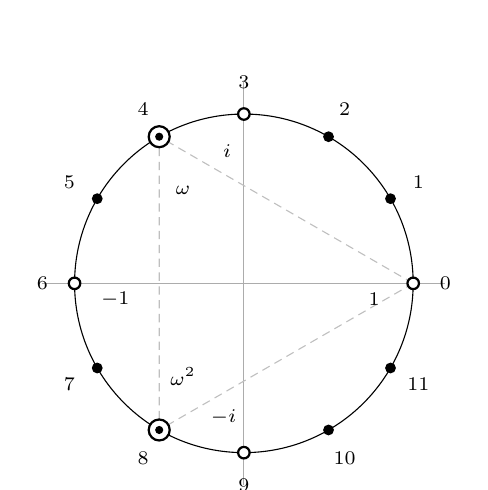
\begin{tikzpicture}[scale=2.15, every node/.style={font=\scriptsize}]
 \draw[thin] (0,0) circle (1);
 \draw[gray!65,thin] (-1.19,0)--(1.19,0);
 \draw[gray!65,thin] (0,-1.19)--(0,1.19);
 \draw[densely dashed,gray!50,thin] (0:1)--(120:1)--(240:1)--cycle;
 \foreach \h in {0,...,11} {
  \coordinate (z\h) at ({30*\h}:1);
  \ifnum\h=0
    \draw[fill=white,thick] (z\h) circle (0.034);
  \else\ifnum\h=3
    \draw[fill=white,thick] (z\h) circle (0.034);
  \else\ifnum\h=6
    \draw[fill=white,thick] (z\h) circle (0.034);
  \else\ifnum\h=9
    \draw[fill=white,thick] (z\h) circle (0.034);
  \else\ifnum\h=4
    \draw[fill=white,thick] (z\h) circle (0.062);
    \fill (z\h) circle (0.024);
  \else\ifnum\h=8
    \draw[fill=white,thick] (z\h) circle (0.062);
    \fill (z\h) circle (0.024);
  \else
    \fill (z\h) circle (0.032);
  \fi\fi\fi\fi\fi\fi
  \node at ({30*\h}:1.19) {$\h$};
 }
 \node at (0.77,-0.095) {$1$};
 \node at (-0.10,0.78) {$i$};
 \node at (-0.76,-0.095) {$-1$};
 \node at (-0.12,-0.79) {$-i$};
 \node at (-0.36,0.55) {$\omega$};
 \node at (-0.36,-0.55) {$\omega^2$};
\end{tikzpicture}
\end{minipage}
\caption{Geometry and multiplicity of the zeros of $P$ on the unit circle.
All twelve possible angles are indexed by $h=0,\ldots,11$, increasing
counterclockwise in steps of $\pi/6$. Four open markers at
$h=0,3,6,9$ represent the nonroots $1,i,-1,-i$; six solid markers
represent simple roots; and two concentric markers at $h=4,8$
represent the double roots $\omega,\omega^2$. The dashed equilateral
triangle connects $1,\omega,\omega^2$ and illustrates the relation
$1+\omega+\omega^2=0$.}
\label{fig:roots}
\end{figure}


Figure~\ref{fig:roots} represents the same index-by-index
multiplicity calculation recorded in Table~\ref{tab:multiplicities}.
The connection follows algebraically from Equation~\eqref{eq:cross-product}.
For $0\leq h<12$, define $\mathbf1_{A}$ to equal one when condition
$A$ holds and zero otherwise. Since
$\omega_{12,h}^{\,r}=1$ exactly when $12$ divides $rh$,
the factor $1-x^{12}$ contributes one zero at every index;
$1-x^3$ contributes one more exactly when $4\mid h$;
$1-x^4$ removes one when $3\mid h$; and $1-x$ removes one
only when $h=0$. Thus Equation~\eqref{eq:cross-product} gives the
explicit index formula
\begin{equation}\label{eq:figure-table-multiplicity}
 \mult_P(\omega_{12,h})
 =1+\mathbf1_{\{4\mid h\}}
  -\mathbf1_{\{3\mid h\}}-\mathbf1_{\{h=0\}},
 \qquad 0\leq h<12.
\end{equation}
For example, Equation~\eqref{eq:figure-table-multiplicity} gives
$1+1-1-1=0$ at $h=0$, $1+0-1-0=0$ at $h=3,6,9$,
$1+1-0-0=2$ at $h=4,8$, and $1+0-0-0=1$ at the six
remaining indices. These are precisely the four rows of
Table~\ref{tab:multiplicities}. The points $h=4,8$ are $\omega$ and $\omega^2$, the two shared
roots of the factors in Equation~\eqref{eq:original-factor}; the dashed
triangle joins them to $1$ and reflects their angular separation
of $2\pi/3$. Complex conjugation maps an index $h$ to $12-h$
modulo twelve, so the diagram is symmetric across the real axis.
The corresponding roots occur in four conjugate pairs, classified by
exact order and algebraic form in Table~\ref{tab:conjugatepairs}.
\begin{table}[H]
\centering
\caption{The eight distinct roots of the original polynomial, arranged
into four complex-conjugate pairs. The order refers to the smallest
positive integer $d$ for which $z^d=1$; the exponential and radical
forms give two representations of each pair. The multiplicity applies
to each root separately, so the four rows represent ten roots when
multiplicity is counted.}
\label{tab:conjugatepairs}
\renewcommand{\arraystretch}{1.42}
\begin{tabular}{@{}cclc@{}}
\toprule
Order & Exponential form & Algebraic form & Multiplicity \\
\midrule
$12$ & $e^{\pm i\pi/6}$ & $\dfrac{\sqrt3\pm i}{2}$ & $1$ \\
$6$ & $e^{\pm i\pi/3}$ & $\dfrac{1\pm i\sqrt3}{2}$ & $1$ \\
$3$ & $e^{\pm 2i\pi/3}$ & $\dfrac{-1\pm i\sqrt3}{2}$ & $2$ \\
$12$ & $e^{\pm 5i\pi/6}$ & $\dfrac{-\sqrt3\pm i}{2}$ & $1$ \\
\bottomrule
\end{tabular}
\end{table}

The first and fourth rows of Table~\ref{tab:conjugatepairs}
contain the primitive twelfth roots; the second contains roots of
order six, and the third contains the primitive cube roots. In the
third row, both members occur twice because the factor $\Phi_3$
appears with exponent two in the rational factorization. Each other
member occurs once, and the degree count is therefore
$2(1+1+2+1)=10$. In particular, the table distinguishes the
\emph{number of displayed complex numbers}, which is eight, from
the \emph{number counted with multiplicity}, which is ten. This
distinction will also enter the coefficient checks below.

\subsection{Relations between roots and coefficients}\label{subsec:viete}

Vi\`ete's formulas express the coefficients of a polynomial in terms of symmetric sums of its complex roots. The roots are listed with multiplicity, so a double root contributes two positions to each sum. The relations follow from the linear factorization established in Equation~\eqref{eq:fta-factorization} and apply regardless of whether the roots have explicit expressions. We introduce the symmetric sums, derive the coefficient identities for an arbitrary leading coefficient, and then recover the quadratic case. The original tenth-degree equation provides a subsequent example in which the coefficient identities can be checked from the root geometry~\cite{barbeau1989,dummit2004}.

\begin{definition}[Elementary symmetric sums]\label{def:symmetric-sums}
Let $r_1,\ldots,r_d\in\C$ be the roots of a polynomial, listed with multiplicity. For $1\leq j\leq d$, the $j$-th \emph{elementary symmetric sum} is the sum of the products of every choice of $j$ distinct indices from this list. With the convention $e_0=1$, the defining expression is
\begin{equation}\label{eq:elementary-symmetric}
 e_j(r_1,\ldots,r_d)=
 \sum_{1\leq i_1<\cdots<i_j\leq d}
 r_{i_1}\cdots r_{i_j},\qquad 1\leq j\leq d.
\end{equation}
Repeated root values occupy different indices and are counted according to their multiplicity.
\end{definition}

For example, $e_1$ adds the $d$ roots, $e_2$ adds the products of all pairs with different indices, and $e_d$ multiplies all $d$ roots. Let $F(x)=a_dx^d+a_{d-1}x^{d-1}+\cdots+a_0$ be a polynomial over $\C$ with $a_d\neq0$. The fundamental theorem of algebra gives a linear factorization in which each root is repeated according to its multiplicity:
\begin{equation}\label{eq:viete-factor-general}
 F(x)=a_d\prod_{j=1}^{d}(x-r_j).
\end{equation}
The coefficient of $x^{d-j}$ in this product is obtained by selecting $j$ factors of the form $-r_i$ and taking $x$ from the other $d-j$ factors. Each selection contributes $(-1)^jr_{i_1}\cdots r_{i_j}$, so comparing coefficients in Equation~\eqref{eq:viete-factor-general} gives the general formulas.

\begin{proposition}[Vi\`ete's formulas]\label{prop:viete}
For $F$ and its roots as above, the coefficients determine the elementary symmetric sums by
\begin{align}
 r_1+\cdots+r_d
   &= -\frac{a_{d-1}}{a_d},\label{eq:viete-first-general}\\
 \sum_{1\leq i<j\leq d}r_ir_j
   &= \frac{a_{d-2}}{a_d},\label{eq:viete-second-general}\\
 e_j(r_1,\ldots,r_d)
   &=(-1)^j\frac{a_{d-j}}{a_d},\qquad 1\leq j\leq d,\label{eq:viete-middle-general}\\
 r_1r_2\cdots r_d
   &=(-1)^d\frac{a_0}{a_d}.\label{eq:viete-last-general}
\end{align}
In particular, for a monic polynomial $a_d=1$, the signs alternate in its expansion:
\begin{equation}\label{eq:viete-expanded}
 F(x)=x^d-e_1x^{d-1}+e_2x^{d-2}-\cdots+(-1)^de_d.
\end{equation}
\end{proposition}
\begin{proof}
Expanding Equation~\eqref{eq:viete-factor-general} and grouping terms with the same power of $x$ gives $a_{d-j}=(-1)^ja_de_j$. Division by $a_d\neq0$ proves Equation~\eqref{eq:viete-middle-general}. Its cases $j=1$, $j=2$, and $j=d$ give Equations~\eqref{eq:viete-first-general}, \eqref{eq:viete-second-general}, and \eqref{eq:viete-last-general}, respectively. Setting $a_d=1$ yields Equation~\eqref{eq:viete-expanded}.
\end{proof}

For a quadratic $q(x)=ax^2+bx+c$ with $a\neq0$, the sums $e_1$ and $e_2$ exhaust all elementary symmetric sums. If $r_1,r_2$ are its roots, Equations~\eqref{eq:viete-first-general} and \eqref{eq:viete-last-general} specialize to
\begin{equation}\label{eq:girard-quadratic}
 r_1+r_2=-\frac{b}{a},\qquad r_1r_2=\frac{c}{a}.
\end{equation}
These are the quadratic case of Vi\`ete's formulas (sometimes attributed to Girard). Indeed, the factorization $q(x)=a(x-r_1)(x-r_2)$ expands to $ax^2-a(r_1+r_2)x+ar_1r_2$; coefficient comparison gives Equation~\eqref{eq:girard-quadratic}. Applying the relations to the quadratic factor $x^2+x+1$ of Equation~\eqref{eq:original-factor}, whose roots are $\omega$ and $\omega^2$, gives
\begin{equation}\label{eq:girard-cube-roots}
 \omega+\omega^2=-1,\qquad \omega\,\omega^2=\omega^3=1.
\end{equation}
The sum in Equation~\eqref{eq:girard-cube-roots} also expresses the three-term identity $1+\omega+\omega^2=0$ used to locate the primitive cube roots of unity. Thus the quadratic coefficient relations and the geometric-series factorization describe the same two roots.

For the original polynomial in Equation~\eqref{eq:original}, the degree is ten, and the coefficients of $x^9$, $x^8$, and $x^0$ all equal one. The monic formula in Equation~\eqref{eq:viete-expanded} therefore requires $e_1=-1$, $e_2=1$, and $e_{10}=1$. The four conjugate pairs in Table~\ref{tab:conjugatepairs} let us check these values without expanding the tenth-degree product. A pair $e^{\pm i\theta}$ has sum $2\cos\theta$ and product one. The pair with angle $2\pi/3$ occurs twice, so the sum of all ten roots, counted with multiplicity, is
\begin{equation}\label{eq:vietecheck}
 \sum_{j=1}^{10}r_j
 =2\cos\frac{\pi}{6}+2\cos\frac{\pi}{3}
  +4\cos\frac{2\pi}{3}+2\cos\frac{5\pi}{6}
 =\sqrt3+1-2-\sqrt3=-1.
\end{equation}
For the coefficient of $x^8$, we use the identity $\bigl(\sum_jr_j\bigr)^2=\sum_jr_j^2+2e_2$, obtained by distinguishing the diagonal terms from the products with unequal indices. Squaring a unit-circle root doubles its argument, so the same four conjugate pairs give
\begin{equation}\label{eq:viete-power-sum}
 \begin{aligned}
 \sum_{j=1}^{10}r_j^2
 &=2\cos\frac{\pi}{3}+2\cos\frac{2\pi}{3}
   +4\cos\frac{4\pi}{3}+2\cos\frac{5\pi}{3}\\
 &=1-1-2+1=-1.
 \end{aligned}
\end{equation}
Combining this result with Equation~\eqref{eq:vietecheck}, the second elementary symmetric sum is
\begin{equation}\label{eq:viete-second-sum}
 e_2=\frac12\left[\left(\sum_{j=1}^{10}r_j\right)^2
                   -\sum_{j=1}^{10}r_j^2\right]
 =\frac{1-(-1)}{2}=1.
\end{equation}
Finally, each conjugate pair has product $e^{i\theta}e^{-i\theta}=1$. Counting the double pair twice gives $e_{10}=\prod_{j=1}^{10}r_j=1$, as required by Equation~\eqref{eq:viete-last-general} for a monic polynomial of even degree. These three checks test coefficients of the polynomial, while the factorization in Equation~\eqref{eq:original-factor} determines the full set of roots and their multiplicities.

\subsection{An independent substitution}\label{subsec:substitution}

The second factor $1+x^4+x^8$ of Equation~\eqref{eq:original-factor} contains powers whose exponents are multiples of four. Its three terms can therefore be expressed through a single variable $u=x^4$, with $x^8=u^2$. This substitution turns the eighth-degree equation into a quadratic equation for $u$. The quadratic has two nonzero complex roots; recovering $x$ then requires finding the four fourth roots of each value. This separates the calculation into a quadratic step followed by a root-extraction step, allowing us to count all eight roots before comparing them with those of the other factor.

Substituting $u=x^4$ into $1+x^4+x^8=0$ gives the quadratic equation $u^2+u+1=0$. The quadratic formula, or Equation~\eqref{eq:girard-cube-roots} together with the root-of-unity representation, identifies its solutions:
\begin{equation}\label{eq:tquad}
 1+u+u^2=0,\qquad u=\frac{-1\pm i\sqrt3}{2}=e^{\pm2\pi i/3}.
\end{equation}
Both values of $u$ in Equation~\eqref{eq:tquad} have modulus one. Writing $x=\rho e^{i\theta}$ with $\rho>0$, the condition $x^4=u$ gives $\rho^4=1$ and hence $\rho=1$. Comparing arguments modulo $2\pi$ yields $4\theta=\pm2\pi/3+2\pi h$ for an integer $h$. Dividing by four gives the complete angular parametrization, with four residue classes of $h$ for each sign:
\begin{equation}\label{eq:substitution-angles}
 x=e^{i\theta},\qquad
 \theta=\pm\frac{\pi}{6}+\frac{h\pi}{2},\qquad h=0,1,2,3.
\end{equation}
Equation~\eqref{eq:substitution-angles} provides four arguments for the positive sign and four for the negative sign. Taking their representatives in $[0,2\pi)$, the two sets are
$\Theta_{+}=\{\pi/6,2\pi/3,7\pi/6,5\pi/3\}$ and
$\Theta_{-}=\{11\pi/6,\pi/3,5\pi/6,4\pi/3\}$.
Within each set, successive arguments differ by $\pi/2$; the sets do not intersect modulo $2\pi$ because the corresponding fourth powers are distinct. They therefore represent the eight distinct roots of the second factor.

The first factor in Equation~\eqref{eq:original-factor} has roots $\omega$ and $\omega^2$. Their arguments $2\pi/3$ and $4\pi/3$ occur in $\Theta_+$ and $\Theta_-$, respectively. Algebraically, $\omega^3=1$ gives $\omega^4=\omega$ and $\omega^8=\omega^2$, so $1+\omega^4+\omega^8=1+\omega+\omega^2=0$ by Equation~\eqref{eq:girard-cube-roots}. The two factors consequently share exactly these two roots. Since each root is simple in each factor, its multiplicity in their product is two, recovering the corresponding entries of Table~\ref{tab:multiplicities}.

\subsection{Real and rational factorization}\label{subsec:real-rational}

A conjugate pair on the unit circle determines a monic real quadratic factor. For a nonreal root $e^{i\theta}$ and its conjugate $e^{-i\theta}$, direct multiplication gives
\begin{equation}\label{eq:conjugate-factor}
 (x-e^{i\theta})(x-e^{-i\theta})=x^2-2x\cos\theta+1.
\end{equation}
Using representatives $\theta=2\pi/3,\pi/3,\pi/6,5\pi/6$ gives the complete factorization over $\R$,
\begin{equation}\label{eq:real-factor}
 P(x)=(x^2+x+1)^2(x^2-x+1)
       (x^2-\sqrt3x+1)(x^2+\sqrt3x+1).
\end{equation}
For each quadratic in Equation~\eqref{eq:real-factor}, the angle $\theta$ is neither $0$ nor $\pi$. Hence $\cos^2\theta<1$, and its discriminant satisfies $4\cos^2\theta-4<0$. Therefore $P$ has no real roots. The factors with coefficients $\pm\sqrt3$ combine to $x^4-x^2+1$, which has integer coefficients and yields the cyclotomic description~\cite{dummit2004}.

The three rational factors were already calculated in the
cyclotomic examples: Equation~\eqref{eq:cyclo-3} gives
$\Phi_3(x)=x^2+x+1$, Equation~\eqref{eq:cyclo-examples} gives
$\Phi_6(x)=x^2-x+1$, and Equation~\eqref{eq:cyclo-more} gives
$\Phi_{12}(x)=x^4-x^2+1$. Substituting these previously derived
expressions into Equation~\eqref{eq:real-factor}, with the conjugate
irrational quadratics combined into $\Phi_{12}$, produces the
factorization over $\Q$:
\begin{equation}\label{eq:cyclotomic-original}
 P(x)=\Phi_3(x)^2\Phi_6(x)\Phi_{12}(x).
\end{equation}
The exponent of $\Phi_3$ identifies the two repeated primitive cube roots, and the degrees $2\cdot2+2+4=10$ provide an algebraic check on the complete solution.

The same rational decomposition can be obtained directly from the
second factor in Equation~\eqref{eq:original-factor}, using elementary
identities. We first write $1+x^4+x^8=(x^4+1)^2-x^4$;
this equality follows by expanding the square, which contributes
$2x^4$, and then subtracting one copy of $x^4$. The result is a
difference of two squares, with terms $x^4+1$ and $x^2$.
Factoring their sum and difference gives the two quartics.
The first quartic splits further because
$(x^2+x+1)(x^2-x+1)=(x^2+1)^2-x^2=x^4+x^2+1$.
Altogether,
\begin{align}
 1+x^4+x^8
 &= (x^4+1)^2-x^4\notag\\
 &= (x^4+x^2+1)(x^4-x^2+1)\notag\\
 &= (x^2+x+1)(x^2-x+1)(x^4-x^2+1).\label{eq:elementary-cyclo}
\end{align}
The final factors in Equation~\eqref{eq:elementary-cyclo} are precisely
$\Phi_3$, $\Phi_6$, and $\Phi_{12}$, identified in
Equations~\eqref{eq:cyclo-3}, \eqref{eq:cyclo-examples}, and
\eqref{eq:cyclo-more}. Multiplying by the first factor
$1+x+x^2=\Phi_3(x)$ from Equation~\eqref{eq:original-factor}
recovers Equation~\eqref{eq:cyclotomic-original}; hence $\Phi_3$
appears twice. The cyclotomic polynomials are irreducible over
$\Q$~\cite[Section~13.6]{dummit2004}, so the resulting expression
is the irreducible rational factorization. Each factor corresponds
to roots of an exact multiplicative order, explaining why its degree
and exponent determine the associated number of roots and their
multiplicities.

The geometric-series identity, the substitution $u=x^4$, and the cyclotomic decomposition provide three complementary ways to identify the same roots and their multiplicities.


\section{Reciprocal reduction and root counts}\label{sec:chebyshev-applications}

This section develops two extensions of the motivating calculation. Section~\ref{subsec:chebyshev} introduces the Chebyshev--Dickson identity needed to express symmetric Laurent powers as ordinary polynomials. Section~\ref{sec:reciprocalmethod} uses that identity for the reciprocal reduction of the tenth-degree polynomial. Section~\ref{sec:realexamples} then turns from the particular equation to general products of finite geometric sums, deriving formulas for repeated and distinct roots together with a parity criterion for the only possible real root.

\subsection{Chebyshev and Dickson polynomials}\label{subsec:chebyshev}

The reciprocal reduction requires only the symmetric combinations $x^j+x^{-j}$. The Chebyshev polynomials of the first kind provide their trigonometric interpretation, while the corresponding Dickson polynomials provide a standard algebraic notation. For $j\ge0$, define $T_j$ by
\begin{equation}\label{eq:cheb-first}
 T_j(\cos\theta)=\cos(j\theta).
\end{equation}
The cosine addition formula gives
\begin{equation}\label{eq:cheb-T-rec}
 T_0(y)=1,\qquad T_1(y)=y,\qquad T_{j+1}(y)=2yT_j(y)-T_{j-1}(y).
\end{equation}
These standard identities are recorded in the Digital Library of Mathematical Functions and in Mason and Handscomb~\cite{dlmfchebyshev,masonhandscomb2003}.

\begin{proposition}[Symmetric powers and Dickson polynomials]\label{prop:cheb-symmetric}
Let $x\in\C^\times$ and put $t=x+x^{-1}$. For every integer $j\ge0$,
\begin{equation}\label{eq:cheb-lift}
 x^j+x^{-j}=D_j(t,1)=2T_j\!\left(\frac{t}{2}\right),
\end{equation}
where $D_j(t,1)$ is the Dickson polynomial of the first kind with parameter $1$. In particular, if $x=e^{i\theta}$, then $t=2\cos\theta$ and $D_j(t,1)=2\cos(j\theta)$.
\end{proposition}
\begin{proof}
Set $W_j=x^j+x^{-j}$. Then $W_0=2$, $W_1=t$, and multiplication by $x+x^{-1}$ gives
\begin{equation}\label{eq:cheb-symmetric-rec}
 W_{j+1}=tW_j-W_{j-1}.
\end{equation}
The polynomials $2T_j(t/2)$ satisfy the same recurrence and initial conditions by Equation~\eqref{eq:cheb-T-rec}. The standard Dickson recurrence $D_0(t,1)=2$, $D_1(t,1)=t$, $D_{j+1}(t,1)=tD_j(t,1)-D_{j-1}(t,1)$ identifies the common polynomial as $D_j(t,1)$~\cite{lidl1993}.
\end{proof}

\subsection{Reciprocal reduction}\label{sec:reciprocalmethod}

The reduction developed here applies to polynomials whose coefficients are symmetric about their middle degree. For a polynomial of even degree, this symmetry makes it possible to pair each positive power of $x$ with the corresponding negative power after division by the appropriate monomial. Proposition~\ref{prop:cheb-symmetric} then converts every pair into a polynomial in the single variable $t=x+x^{-1}$. Definition~\ref{def:reciprocal} supplies the reciprocal symmetry used here. We specify the domain of the substitution and use Dickson polynomials to convert the symmetric Laurent powers into ordinary polynomials. These steps lead to a fifth-degree polynomial whose factorization can be checked by ordinary algebra and then lifted back to quadratic factors in $x$~\cite{barbeau1989,needham1997,lidl1993}.

The original polynomial $P$ has degree ten, leading coefficient one, and constant coefficient one. Its remaining coefficients are paired symmetrically, as in Equation~\eqref{eq:original}. Consequently, Definition~\ref{def:reciprocal} gives $x^{10}P(x^{-1})=P(x)$ for $x\ne0$. Because $P(0)=1$, no root is lost by restricting the equation to nonzero complex numbers. Dividing by $x^5$ produces a Laurent polynomial invariant under $x\mapsto x^{-1}$. Grouping terms with equal absolute exponents gives
\begin{equation}\label{eq:reciprocal-decomposition}
 x^{-5}P(x)=(x^5+x^{-5})+(x^4+x^{-4})+(x^3+x^{-3})+(x+x^{-1})+1.
\end{equation}

To replace the symmetric powers in Equation~\eqref{eq:reciprocal-decomposition}, set $t=\tau(x):=x+x^{-1}$ for $x\in\C^\times$. Proposition~\ref{prop:cheb-symmetric} gives $D_j(t,1)=x^j+x^{-j}$. The recurrence therefore yields
\begin{subequations}\label{eq:reciprocal-V}
\begin{align}
 D_0(t,1)&=2,\label{eq:reciprocal-D0}\\
 D_1(t,1)&=t,\label{eq:reciprocal-D1}\\
 D_2(t,1)&=t^2-2,\label{eq:reciprocal-D2}\\
 D_3(t,1)&=t^3-3t,\label{eq:reciprocal-D3}\\
 D_4(t,1)&=t^4-4t^2+2,\label{eq:reciprocal-D4}\\
 D_5(t,1)&=t^5-5t^3+5t.\label{eq:reciprocal-D5}
\end{align}
\end{subequations}

We now substitute the computed Dickson polynomials into Equation~\eqref{eq:reciprocal-decomposition}. The $D_2$ term does not appear in that decomposition, so the reduced expression is $D_5+D_4+D_3+D_1+1$, with parameter $1$ understood. Combining equal powers of $t$ yields a monic polynomial of degree five:
\begin{subequations}\label{eq:reduced-quintic}
\begin{equation}\label{eq:reduced-quintic-expanded}
 x^{-5}P(x)=t^5+t^4-4t^3-4t^2+3t+3.
\end{equation}

The coefficients in Equation~\eqref{eq:reduced-quintic-expanded} occur in pairs: the terms of degrees five and four have coefficient one, those of degrees three and two have coefficient minus four, and the terms of degrees one and zero have coefficient three. Factoring $t+1$ from the resulting groups gives
\begin{equation}\label{eq:reduced-quintic-grouped}
 x^{-5}P(x)=(t+1)(t^4-4t^2+3).
\end{equation}

The remaining quartic is a quadratic polynomial in $t^2$. Setting $s=t^2$ gives $s^2-4s+3=(s-1)(s-3)$, so $t^4-4t^2+3=(t^2-1)(t^2-3)$. Factoring the difference of squares $t^2-1=(t-1)(t+1)$ supplies the final factorization:
\begin{equation}\label{eq:reduced-quintic-factored}
 x^{-5}P(x)=(t+1)^2(t-1)(t^2-3).
\end{equation}
\end{subequations}

Define $R(t):=(t+1)^2(t-1)(t^2-3)$ from Equation~\eqref{eq:reduced-quintic-factored}. Its zeros are $t=-1$ with multiplicity two and $t\in\{1,\sqrt3,-\sqrt3\}$ with multiplicity one. To reconstruct the original polynomial, we must relate each linear factor of $R$ to an equation for $x$ rather than treating the values of $t$ as roots of $P$. For a fixed value $t_0\in\C$ and $x\ne0$, the definition $t=x+x^{-1}$ gives
\begin{equation}\label{eq:reciprocal-lift}
 t-t_0=x^{-1}(x^2-t_0x+1).
\end{equation}

The identity in Equation~\eqref{eq:reciprocal-lift} shows that a linear factor $t-t_0$ corresponds to the quadratic polynomial $x^2-t_0x+1$. Inserting all five linear factors of $R$ into $P(x)=x^5R(x+x^{-1})$, the five factors $x^{-1}$ cancel the prefactor $x^5$. The double factor $t+1$ yields $ (x^2+x+1) ^2$, while the single factor $t-1$ yields $x^2-x+1$. The two values $t_0=\pm\sqrt3$ produce the last two quadratics. Therefore
\begin{equation}\label{eq:reciprocal-factor}
 P(x)=(x^2+x+1)^2(x^2-x+1)(x^2-\sqrt3x+1)(x^2+\sqrt3x+1).
\end{equation}

For every $t_0\in\{-1,1,\sqrt3,-\sqrt3\}$, the discriminant of $x^2-t_0x+1$ is $t_0^2-4<0$. Thus each quadratic has two distinct nonreal roots, and different values of $t_0$ give quadratics with disjoint root sets: a common nonzero root would imply the same value $x+x^{-1}=t_0$ for two different constants. Consequently, the multiplicity of $t_0$ in $R$ is inherited by each corresponding root of $P$. The roots associated with $t_0=-1$ are double, and the remaining six roots are simple, consistent with the earlier factorization in Equation~\eqref{eq:real-factor}. Proposition~\ref{prop:cheb-symmetric} also explains the trigonometric content of this construction: when $x=e^{i\theta}$, the reciprocal variable is $t=2\cos\theta$ and the Dickson identity gives $D_j(t,1)=2\cos(j\theta)$. The algebraic reduction and the angular description in Section~\ref{sec:roots} therefore identify the same complex zeros.

\subsection{Root counts and real roots}\label{sec:realexamples}

The motivating polynomial suggests a general question: how many roots are shared by two finite geometric sums, and when can their product have a real zero? The cyclotomic description in Corollary~\ref{cor:geomsum-cyclotomic} answers both questions by reducing them to intersections of finite sets of roots of unity.

\begin{proposition}[Geometric sums of unequal lengths]\label{prop:application-unequal}
Let $m,n\ge2$ and $b\ge1$. The product $Q_{m,n,b}(x)=S_m(x)S_n(x^b)$ has
\begin{subequations}\label{eq:unequal-counts}
\begin{align}
 \delta_{m,n,b}&=\gcd(m,nb)-\gcd(m,b) &&\text{double roots},\label{eq:unequal-double}\\
 \nu_{m,n,b}&=(m-1)+b(n-1)-\delta_{m,n,b} &&\text{distinct roots}.\label{eq:unequal-distinct}
\end{align}
\end{subequations}
All remaining roots are simple, and all roots lie on the unit circle.
\end{proposition}
\begin{proof}
By Corollary~\ref{cor:geomsum-cyclotomic}, the zero sets are $A=\mathcal U_m\setminus\{1\}$ and $B=\mathcal U_{nb}\setminus\mathcal U_b$. Their intersection is $\mathcal U_{\gcd(m,nb)}\setminus\mathcal U_{\gcd(m,b)}$. Since $\gcd(m,b)\mid\gcd(m,nb)$, its cardinality is the difference of these greatest common divisors. Each factor has simple zeros, so the common zeros are exactly the double zeros of the product. Inclusion--exclusion gives the distinct-root count. This is the root-set form of the finite geometric-series greatest-common-divisor formula; compare Hartwig and Patr\'icio~\cite[Lemma~3.3, p.~9976; Theorem~3.4, p.~9977]{hartwig2023gcd}.
\end{proof}

\begin{corollary}[Equal-length products]\label{cor:application-count}
Let $m,b\ge2$ and put $g=\gcd(m,b)$. Then $P_{m,b}(x)=S_m(x)S_m(x^b)$ has $m-g$ double roots and $b(m-1)+g-1$ distinct roots; every other root is simple.
\end{corollary}
\begin{proof}
Set $n=m$ in Proposition~\ref{prop:application-unequal}. Since $\gcd(m,mb)=m$, Equation~\eqref{eq:unequal-double} becomes $m-\gcd(m,b)$, and Equation~\eqref{eq:unequal-distinct} gives the stated count.
\end{proof}

\begin{proposition}[Parity criterion for real roots]\label{prop:real-parity}
For $Q_{m,n,b}(x)=S_m(x)S_n(x^b)$, a real root exists if and only if $m$ is even, or $n$ is even and $b$ is odd. When it exists, $x=-1$ is the unique real root. It is double exactly when $m$ and $n$ are even and $b$ is odd; otherwise it is simple. If no real root exists, then $Q_{m,n,b}(x)>0$ for all $x\in\R$.
\end{proposition}
\begin{proof}
All zeros lie on the unit circle by Proposition~\ref{prop:application-unequal}, so a real zero can only be $\pm1$. Since $S_r(1)=r>0$, the value $1$ is never a zero. Moreover,
\begin{equation}\label{eq:parity-sum}
 S_r(-1)=\begin{cases}0,&r\text{ even},\\1,&r\text{ odd}.\end{cases}
\end{equation}
Thus the first factor vanishes at $-1$ exactly when $m$ is even. The second factor vanishes there exactly when $b$ is odd and $n$ is even. Each factor has only simple zeros, so the multiplicity is the number of vanishing factors. If neither factor has a real zero, continuity and the positive value at zero show that each remains positive on $\R$.
\end{proof}

For the motivating polynomial, the factorization in Equation~\eqref{eq:original-factor} is precisely
\begin{equation}\label{eq:original-family}
 P(x)=S_3(x)S_3(x^4)=P_{3,4}(x).
\end{equation}
Corollary~\ref{cor:application-count} therefore predicts two double roots and eight distinct roots before any individual root is listed, in agreement with Section~\ref{subsec:counts} and Table~\ref{tab:twofactorcases}.

\subsection{Example: \texorpdfstring{$m=4$, $b=2$}{m=4, b=2}}\label{ex:fourtwo}

We first choose $m=4$ and $b=2$ to examine a product in which the two factors have some common zeros, but neither zero set contains the other. The parameters specify a geometric sum of four consecutive powers and a second sum obtained by replacing $x$ with $x^2$. Their lengths are equal, but their exponent spacings are different. Before performing any factorization, Corollary~\ref{cor:application-count} gives $g=\gcd(4,2)=2$, predicts $m-g=2$ double zeros, and gives $b(m-1)+g-1=7$ distinct zeros in a polynomial of degree $(m-1)(b+1)=9$. We now identify these zeros through the cyclotomic factors and verify the predicted count.

By the definition of the finite geometric sum, the first factor is
\begin{subequations}\label{eq:example-fourtwo}
\begin{equation}\label{eq:example-fourtwo-first}
 S_4(x)=1+x+x^2+x^3.
\end{equation}
Replacing $x$ by $x^2$ gives the dilated factor,
\begin{equation}\label{eq:example-fourtwo-second}
 S_4(x^2)=1+x^2+x^4+x^6.
\end{equation}
The product of the factors in Equations~\eqref{eq:example-fourtwo-first} and~\eqref{eq:example-fourtwo-second} is therefore
\begin{equation}\label{eq:example-fourtwo-expanded}
 P_{4,2}(x)=S_4(x)S_4(x^2)=(1+x+x^2+x^3)(1+x^2+x^4+x^6).
\end{equation}

Corollary~\ref{cor:geomsum-cyclotomic} gives $S_4(x)=\Phi_2(x)\Phi_4(x)$. Similarly, $S_4(x^2)=(x^8-1)/(x^2-1)$ contains the factors of $x^8-1$ whose orders do not divide two, so $S_4(x^2)=\Phi_4(x)\Phi_8(x)$. Multiplying these two decompositions gives
\begin{equation}\label{eq:example-fourtwo-cyclotomic}
 P_{4,2}(x)=\Phi_2(x)\Phi_4(x)^2\Phi_8(x).
\end{equation}

The square on $\Phi_4$ is caused by its occurrence in both geometric sums. The explicit formulas $\Phi_2(x)=x+1$, $\Phi_4(x)=x^2+1$, and $\Phi_8(x)=x^4+1$, obtained in Section~\ref{sec:rootsunity}, now yield the factorization over $\Q$:
\begin{equation}\label{eq:example-fourtwo-factored}
 P_{4,2}(x)=(x+1)(x^2+1)^2(x^4+1).
\end{equation}
\end{subequations}

The factors in Equation~\eqref{eq:example-fourtwo-factored} classify the solutions by their exact orders. The equation $x+1=0$ contributes the order-two root $-1$, with multiplicity one. The equation $x^2+1=0$ contributes the order-four roots $i$ and $-i$; both are double roots because the polynomial factor appears with exponent two. Finally, $x^4+1=0$ implies $x^8=1$ and $x^4\ne1$, so its solutions are the four primitive eighth roots with arguments $\{\pi/4,3\pi/4,5\pi/4,7\pi/4\}$, each simple. The three groups are disjoint because a root of unity has one exact multiplicative order. We obtain five simple roots and two double roots: the seven distinct roots account for $5+2\cdot2=9$ roots with multiplicity, matching the degree computed from Equation~\eqref{eq:example-fourtwo-expanded}. Figure~\ref{fig:fourtwo} represents the same classification geometrically.

\begin{figure}[H]
\centering
\begin{minipage}[c]{0.53\textwidth}
\small\setlength{\parindent}{1em}
The points in the diagram are the eight solutions of $x^8=1$, spaced by an angle of $\pi/4$. The identity $S_4(x^2)=(x^8-1)/(x^2-1)$ excludes the points $1$ and $-1$, while $S_4(x)$ contributes $-1$, $i$, and $-i$. Hence the union of the two factor zero sets consists of every eighth root of unity except $1$. The two roots $\{i,-i\}$ belong to both factors and have multiplicity two. The point $-1$ belongs only to the first factor and is simple. The four diagonal vertices are simple roots of the second factor. Filled, open, and concentric markers indicate these distinctions.
\end{minipage}\hfill
\begin{minipage}[c]{0.43\textwidth}
\centering
\begin{tikzpicture}[scale=1.50,every node/.style={font=\scriptsize}]
 \draw[gray!65,thin] (0,0) circle (1);
 \draw[gray!60,thin] (-1.19,0)--(1.19,0) (0,-1.19)--(0,1.19);
 \foreach \h in {0,...,7}{
  \coordinate (v\h) at ({45*\h}:1);
  \ifnum\h=0\draw[fill=white] (v\h) circle (0.046);
  \else
    \ifnum\h=2\draw (v\h) circle (0.084);\fi
    \ifnum\h=6\draw (v\h) circle (0.084);\fi
    \fill (v\h) circle (0.027);
  \fi
 }
 \node[right] at (1.12,0) {$1$};
 \node[left] at (-1.10,0) {$-1$};
 \node[above] at (0,1.12) {$i$};
 \node[below] at (0,-1.12) {$-i$};
\end{tikzpicture}
\end{minipage}
\caption{Complex roots of $P_{4,2}(x)=S_4(x)S_4(x^2)$ and their multiplicities. The open marker at $1$ marks an excluded eighth root of unity; a filled marker denotes a root of the product. The outer rings at $i$ and $-i$ mark the two common roots, each of multiplicity two. The remaining five filled points represent simple zeros, including the real root $-1$. The explanatory text on the left derives these classes from the factor zero sets.}
\label{fig:fourtwo}
\end{figure}

\subsection{Example: \texorpdfstring{$m=b=3$}{m=b=3}}\label{ex:threethree}

The second example chooses the exponent spacing equal to the number of terms in each geometric sum. For $m=b=3$, the first factor contains the powers $x^0,x^1,x^2$, and the second contains $x^0,x^3,x^6$. Multiplying them produces consecutive exponents from zero through eight, with no overlap between distinct pairs of summation indices. At the level of roots, Corollary~\ref{cor:application-count} gives $g=\gcd(3,3)=3=m$, so the predicted number of double roots is $m-g=0$. The example therefore shows how the exponent pattern and the root-set intersection can be analyzed separately and then reconciled by factorization.

The defining product and its expanded geometric sums are
\begin{subequations}\label{eq:example-threethree}
\begin{equation}\label{eq:example-threethree-expanded}
 P_{3,3}(x)=S_3(x)S_3(x^3)=(1+x+x^2)(1+x^3+x^6).
\end{equation}

The first factor vanishes at the two primitive cube roots of unity. Corollary~\ref{cor:geomsum-cyclotomic} gives $S_3(x)=\Phi_3(x)$. The second factor satisfies $S_3(x^3)=(x^9-1)/(x^3-1)$; the numerator contains all cyclotomic factors associated with divisors of nine, while the denominator removes the factors of orders one and three. Only the factor of order nine remains. Thus
\begin{equation}\label{eq:example-threethree-cyclotomic}
 P_{3,3}(x)=\Phi_3(x)\Phi_9(x).
\end{equation}

To relate this factorization to the coefficient pattern, use the finite geometric-series identity in Equation~\eqref{eq:geomsum-basic}. The intermediate factor $x^3-1$ cancels, and the quotient by $x-1$ is the sum of all powers from zero to eight:
\begin{equation}\label{eq:example-threethree-geometric}
 P_{3,3}(x)=\frac{x^9-1}{x-1}=S_9(x)=1+x+x^2+\cdots+x^8.
\end{equation}
\end{subequations}

The factors in Equation~\eqref{eq:example-threethree-cyclotomic} identify two roots of exact order three and six of exact order nine. Explicitly, the first pair is $\{e^{2\pi i/3},e^{4\pi i/3}\}$, while the second group is $\{e^{2\pi i h/9}:h\in\{1,2,4,5,7,8\}\}$. None can occur in both groups because multiplicative order is unique. The polynomial has degree eight, eight distinct roots, and no repeated roots. The same conclusion follows directly from Equation~\eqref{eq:example-threethree-geometric}: $S_9(x)$ vanishes at every ninth root of unity except one, and all these zeros are simple. Comparing this example with $P_{3,4}$ makes the role of the spacing parameter explicit: when $b=3$, $g=m$ eliminates common roots; when $b=4$, $g=1$ produces two common zeros, even though both products have coefficients in $\{0,1\}$.

The root counts for four parameter choices are recorded in Table~\ref{tab:twofactorcases}. The count of double roots is $m-\gcd(m,b)$; the number of distinct roots follows from subtracting these common roots from the sum of the two factor degrees. Both identities are established in Corollary~\ref{cor:application-count}, without computing the individual roots.
\begin{table}[H]
\centering
\caption{Root classification for four products $P_{m,b}(x)=S_m(x)S_m(x^b)$. Here $g=\gcd(m,b)$, $\deg P_{m,b}=(m-1)(b+1)$, the double-root count is $m-g$, the distinct-root count is $b(m-1)+g-1$, and the simple-root count is their difference. The final column records whether the product has a real root and, if so, its multiplicity.}
\label{tab:twofactorcases}
\renewcommand{\arraystretch}{1.52}
\begin{tabular*}{\textwidth}{@{}@{\extracolsep{\fill}}cccccccc@{}}
\toprule
$m$ & $b$ & $g$ & $\deg P_{m,b}$ & Distinct & Simple & Double & Real root\\
\midrule
$3$ & $4$ & $1$ & $10$ & $8$ & $6$ & $2$ & none\\
$4$ & $2$ & $2$ & $9$ & $7$ & $5$ & $2$ & $-1$ (simple)\\
$3$ & $3$ & $3$ & $8$ & $8$ & $8$ & $0$ & none\\
$5$ & $6$ & $1$ & $28$ & $24$ & $20$ & $4$ & none\\
\bottomrule
\end{tabular*}
\end{table}

Table~\ref{tab:twofactorcases} makes the distinction between algebraic degree, distinct roots, and root multiplicity explicit. The degree counts every root with its multiplicity, whereas the distinct-root column counts each location on the unit circle once. For a product with only simple and double zeros, the number of simple roots equals the distinct-root count minus the double-root count; consequently, $\deg P_{m,b}=\text{Simple}+2\,\text{Double}$. For $(m,b)=(4,2)$, the values are $5+2\cdot2=9$: the two double roots are $i$ and $-i$, and the real root $-1$ is simple, as indicated in Figure~\ref{fig:fourtwo}. For $(3,3)$, $g=m$ and no roots are shared, so all eight roots are simple. For $(3,4)$, the two nontrivial cubic roots are shared, and six additional roots are simple. Finally, $(5,6)$ gives $20$ simple and $4$ double roots, accounting for all $28$ occurrences. A real root can only be $-1$, because every root has modulus one and $P_{m,b}(1)=m^2>0$; it occurs when $m$ is even, and its multiplicity is determined by whether $b$ is odd or even. Thus the final column provides a parity check independent of the degree count.



\section{Worked exercises}\label{sec:exercise-section}

The preceding sections establish three methods for studying products of finite geometric sums. Cyclotomic factorization identifies the multiplicative orders of their roots, intersections of root sets determine repeated zeros, and degree counts verify the resulting multiplicities. The following three worked exercises apply these methods to products with equal and unequal numbers of terms. Each example is followed by a solution and a brief remark identifying the general principle used.

\subsection{A product of two three-term sums}\label{subsec:exercise-one}

Our first application retains the three-term geometric sum that appears in the original tenth-degree equation, but replaces the exponent step four with the smaller step two. This modification changes the ambient set of roots from the twelfth to the sixth roots of unity. The analysis therefore begins with the cyclotomic decomposition of the two factors and proceeds to the multiplicities of their common roots. In particular, one must distinguish the \emph{order} of a root, which is the smallest positive exponent sending it to one, from its \emph{multiplicity} as a zero of the product. The two quantities describe different properties of the same complex number, and both are needed to classify the solutions.

\begin{example}[A product of degree six]\label{exercise:one}
The polynomial
\begin{equation}\label{eq:exercise1-polynomial}
 F_1(x)=(1+x+x^2)(1+x^2+x^4)
\end{equation}
has cyclotomic factorization $F_1(x)=\Phi_3(x)^2\Phi_6(x)$. Its four distinct roots consist of two primitive cube roots, each of multiplicity two, and two primitive sixth roots, each of multiplicity one. Their multiplicities sum to $\deg F_1=6$.
\end{example}
\begin{proof}[Solution]
By Equation~\eqref{eq:geomsum-telescoping}, the first factor is the quotient $(x^3-1)/(x-1)$. The cyclotomic factorization $x^3-1=\Phi_1(x)\Phi_3(x)$ and the identity $\Phi_1(x)=x-1$ imply $1+x+x^2=\Phi_3(x)$. To treat the second factor, apply the same geometric-series identity with the substitution $x\mapsto x^2$. The corresponding quotient is $(x^6-1)/(x^2-1)$. Its numerator is the product of the cyclotomic polynomials indexed by the positive divisors of six, while its denominator contains the factors indexed by the divisors of two. Cancellation therefore gives the separate identities
\begin{subequations}\label{eq:exercise1-factors}
\begin{align}
 &1+x+x^2=\frac{x^3-1}{x-1}=\Phi_3(x),\label{eq:exercise1-first}\\
 &1+x^2+x^4=\frac{x^6-1}{x^2-1}=\Phi_3(x)\Phi_6(x).\label{eq:exercise1-second}
\end{align}
\end{subequations}
Multiplying Equations~\eqref{eq:exercise1-first} and \eqref{eq:exercise1-second} establishes the factorization
\begin{equation}\label{eq:exercise1}
 F_1(x)=\Phi_3(x)^2\Phi_6(x).
\end{equation}
By Definition~\ref{def:order}, a primitive $d$-th root of unity has multiplicative order exactly $d$. The zeros of $\Phi_3$ are therefore $\omega_{3,1}=e^{2\pi i/3}$ and $\omega_{3,2}=e^{4\pi i/3}$, while those of $\Phi_6$ are $\omega_{6,1}=e^{\pi i/3}$ and $\omega_{6,5}=e^{5\pi i/3}$. These two pairs are disjoint because a complex root of unity has a unique order. Each factor $\Phi_d$ has simple roots, so the exponent two on $\Phi_3$ makes each primitive cube root a double root of $F_1$, whereas the single factor $\Phi_6$ contributes two simple roots. Thus the distinct-root count is $2+2=4$, and counting with multiplicities gives $2(2)+2(1)=6$. This equals $\deg(1+x+x^2)+\deg(1+x^2+x^4)=2+4$, as required.
\end{proof}

\begin{remark}[Application of the factorization]\label{rem:exercise-one}
The substitution $x\mapsto x^2$ changes the second factor's root set to $\mathcal U_6\setminus\mathcal U_2$, but the primitive cube roots remain zeros of both factors. Equation~\eqref{eq:exercise1} records this overlap through the square $\Phi_3^2$. The calculation shows how cyclotomic factorization simultaneously gives the roots' locations, orders, and multiplicities, without solving a sixth-degree equation by radicals.
\end{remark}

\subsection{Counting roots from a greatest common divisor}\label{subsec:exercise-two}

The next product has a higher degree, but we can determine its root counts before listing any individual root. The essential input is the intersection of two finite sets of roots of unity. In a product of two geometric sums of the same length, each factor has only simple zeros; a repeated zero of the product must therefore occur in both sets. Corollary~\ref{cor:application-count} expresses the size of their intersection in terms of the greatest common divisor of the geometric-series length and the exponent step. We apply the formula to the degree-twenty-five product, then identify which roots are shared and examine the only possible real zero.

\begin{example}[Root counts for $P_{6,4}$]\label{exercise:two}
For $P_{6,4}(x)=S_6(x)S_6(x^4)$, the degree is $25$. The polynomial has $21$ distinct roots: $4$ are double, and $17$ are simple. Its only real root is $x=-1$, and that root is simple.
\end{example}
\begin{proof}[Solution]
The geometric sum $S_6(x)$ has degree five, while $S_6(x^4)$ has degree $4(6-1)=20$. Since both polynomials are monic, their product has degree $5+20=25$. To determine which zeros are repeated, define $g=\gcd(6,4)=2$. Corollary~\ref{cor:application-count} gives $6-g=4$ common zeros, each of multiplicity 2, since the two factors have simple roots. The same corollary gives $4(6-1)+g-1=21$ distinct zeros. Subtracting the four double roots from the distinct-root count leaves seventeen simple roots. These calculations may be written together as
\begin{subequations}\label{eq:exercise2-counts}
\begin{align}
 &\deg P_{6,4}=(6-1)(4+1)=25,\label{eq:exercise2-degree}\\
 &N_{\mathrm{double}}=6-\gcd(6,4)=4,\label{eq:exercise2-double}\\
 &N_{\mathrm{distinct}}=4(6-1)+\gcd(6,4)-1=21,\label{eq:exercise2-distinct}\\
 &N_{\mathrm{simple}}=21-4=17.\label{eq:exercise2-simple}
\end{align}
\end{subequations}
The common-root interpretation makes the count explicit. The first factor vanishes on $\mathcal U_6\setminus\{1\}$, and the second vanishes on $\mathcal U_{24}\setminus\mathcal U_4$. Their intersection is $\mathcal U_6\setminus\mathcal U_4$, which equals $\mathcal U_6\setminus\mathcal U_2$ because $\mathcal U_6\cap\mathcal U_4=\mathcal U_2$. Hence the four double roots are $\{\omega_{6,h}:h\in\{1,2,4,5\}\}$; they comprise two roots of order six and two of order three. Every root of either factor is a root of unity, so any real root must equal $1$ or $-1$. The first value is excluded because $P_{6,4}(1)=S_6(1)^2=36$. At $x=-1$, the alternating sum $S_6(-1)$ equals zero, whereas $S_6((-1)^4)=S_6(1)=6$. Thus only the first factor vanishes at $-1$, and it does so simply. No other real root exists. Finally, the root counts satisfy $17+2\cdot4=25$, independently verifying the algebraic degree.
\end{proof}

\begin{remark}[Application of the counting formulas]\label{rem:exercise-two}
This example separates three different counts: degree, distinct roots, and double roots. The value $\gcd(6,4)=2$ determines the overlap of the zero sets without requiring a factorization of the degree-twenty-five product into irreducible factors. The parity calculation at $-1$ then identifies its real-root multiplicity, providing an additional check on the general count.
\end{remark}

\subsection{An unequal-length product with shared roots}\label{subsec:exercise-four}

The final exercise combines the preceding techniques in a product whose factors have different lengths and different exponent spacings. We choose $m=6$, $n=4$, and $b=3$ so that the first factor has zeros among the sixth roots of unity while the second factor has zeros among the twelfth roots, excluding the cube roots. The difference of two greatest common divisors, established in Proposition~\ref{prop:application-unequal}, gives the number of shared roots. We then determine their positions, classify their orders, and use the degree to verify that we have counted every root with the correct multiplicity.

\begin{example}[A product with two different lengths]\label{exercise:four}
For $Q_{6,4,3}(x)=S_6(x)S_4(x^3)$, there are three distinct double roots and eleven distinct roots in total. The double roots are $e^{\pi i/3}$, $-1$, and $e^{5\pi i/3}$, of orders six, two, and six, respectively. There are eight simple roots, and the total multiplicity equals the degree $14$.
\end{example}
\begin{proof}[Solution]
The first factor $S_6(x)$ has degree $6-1=5$, while the substituted factor $S_4(x^3)$ has degree $3(4-1)=9$. Thus $\deg Q_{6,4,3}=5+9=14$. According to Proposition~\ref{prop:application-unequal}, the number of double roots is the difference between $\gcd(m, nb)$ and $\gcd(m,b)$. In this case $nb=4\cdot3=12$, so the two greatest common divisors are $\gcd(6,12)=6$ and $\gcd(6,3)=3$. The double-root count is therefore $6-3=3$. The total number of distinct roots is the sum of the numbers of roots of the two factors, less these three common roots. Explicitly,
\begin{subequations}\label{eq:exercise4-counts}
\begin{align}
 &\delta_{6,4,3}=\gcd(6,12)-\gcd(6,3)=6-3=3,\label{eq:exercise4-double}\\
 &\nu_{6,4,3}=(6-1)+3(4-1)-\delta_{6,4,3}=5+9-3=11.\label{eq:exercise4}
\end{align}
\end{subequations}
To identify the double roots, examine the two zero sets. The first factor contributes $\mathcal U_6\setminus\{1\}$, and the second contributes $\mathcal U_{12}\setminus\mathcal U_3$. Since $\mathcal U_6\subseteq\mathcal U_{12}$ and $\mathcal U_3\subseteq\mathcal U_6$, their intersection is $\mathcal U_6\setminus\mathcal U_3$. In terms of the indexed roots $\omega_{6,h}=e^{2\pi i h/6}$, this intersection is
\begin{equation}\label{eq:exercise4-common-roots}
 \mathcal U_6\setminus\mathcal U_3=\{\omega_{6,1},\omega_{6,3},\omega_{6,5}\}=\{e^{\pi i/3},-1,e^{5\pi i/3}\}.
\end{equation}
The order of $e^{\pi i/3}$ is six, because its first positive integer power equal to one is its sixth power. The same holds for $e^{5\pi i/3}$, whereas $-1$ has order two. Both factors have simple zeros, so each member of the intersection in Equation~\eqref{eq:exercise4-common-roots} occurs twice in the product. The remaining $11-3=8$ distinct roots are simple. Counting occurrences gives $8+2\cdot3=14$, which equals the degree computed at the beginning of the solution. In addition, $-1$ is a double real root: both $S_6(-1)$ and $S_4((-1)^3)=S_4(-1)$ vanish, agreeing with the parity criterion of Proposition~\ref{prop:real-parity}.
\end{proof}

\begin{remark}[Application of the root-set intersection]\label{rem:exercise-four}
The subtraction $\gcd(6,12)-\gcd(6,3)$ removes from the sixth roots of unity the three roots also belonging to $\mathcal U_3$, because those values do not annihilate the second geometric sum. The resulting set identifies all repeated roots and explains their orders. The degree check and the parity criterion provide independent confirmations of the count and of the double real root.
\end{remark}

\section{Conclusion}\label{sec:conclusion}

The motivating tenth-degree polynomial is recognized from its exponent blocks as $P(x)=S_3(x)S_3(x^4)=P_{3,4}(x)$. Its cyclotomic factorization $P=\Phi_3^2\Phi_6\Phi_{12}$ gives eight distinct roots: six simple roots and two double roots, the primitive cube roots. The unit-circle geometry, the substitution $u=x^4$, Vi\`ete's formulas, and the reciprocal reduction through Dickson polynomials provide independent descriptions and checks of the same solution.

The more general result concerns $Q_{m,n,b}(x)=S_m(x)S_n(x^b)$. Proposition~\ref{prop:application-unequal} shows that the number of shared, hence double, zeros is $\gcd(m,nb)-\gcd(m,b)$ and that the number of distinct zeros is $(m-1)+b(n-1)$ minus this overlap. Corollary~\ref{cor:application-count} recovers the equal-length family, including the original polynomial. Proposition~\ref{prop:real-parity} complements these counts with a complete criterion for the only possible real root: $-1$ occurs exactly under the stated parity conditions and is double precisely when both geometric factors vanish there. These formulas isolate the structural content of the examples and explain how multiplicity is controlled by intersections of root-of-unity sets.

\bibliographystyle{unsrt}
\bibliography{references}
\end{document}
